%!TEX root = ../thesis.tex
% ******************************* Thesis Appendix A ****************************
\chapter{Appendix A: Supplemental data} 


\graphicspath{{Appendix1/Figs/Raster/}{Appendix1/Figs/PDF/}{Appendix1/Figs/}}


\section{Supplemental SEM images}


\begin{figure}[H]
\centering
\begin{minipage}{.45\textwidth}
  \centering
  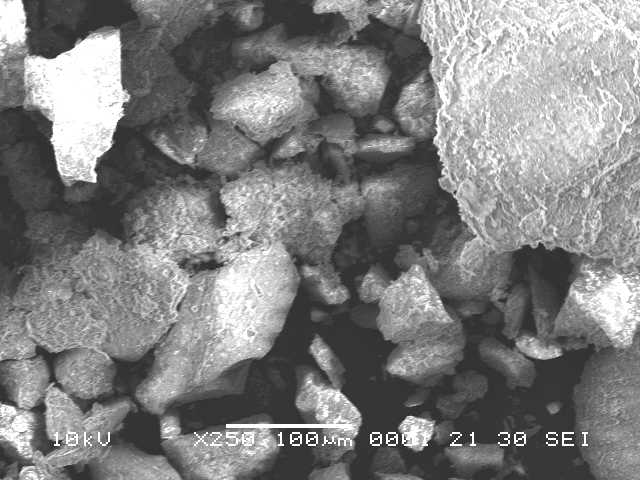
\includegraphics[width=\linewidth]{HKI_natural_azurite_x250_3_040521}
\end{minipage}
\begin{minipage}{.45\textwidth}
  \centering
  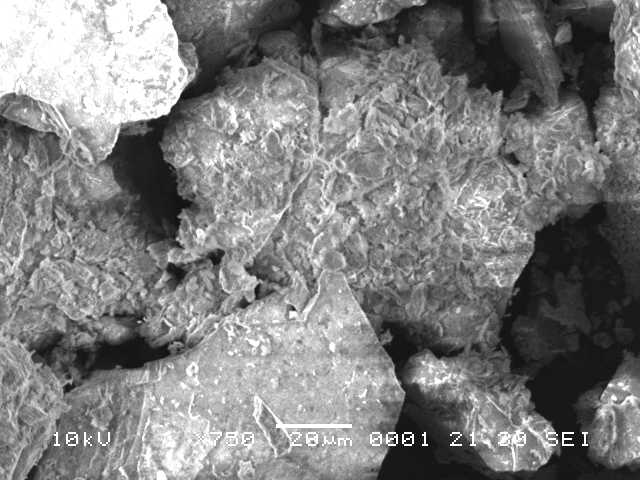
\includegraphics[width=\linewidth]{HKI_natural_azurite_x750_1_040521}
\end{minipage}
\caption[SEM images: Sample HKI, natural azurite]{SEM images: Sample HKI, natural azurite. Magnification: \textbf{left)} 250x, \textbf{right)} 750x.}
\label{fig:hki_nat_az_sem_3}
\end{figure}

The fine surface detail on the flat sides of larger particles in HKI natural azurite can be observed at 1500x magnification in \textit{Figure \ref{fig:hki_nat_az_sem_4}}. The image on the right shows several more spherical looking particles, though many more appear asymmetrical with uneven sharp edges. 

\begin{figure}[H]
\centering
\begin{minipage}{.45\textwidth}
  \centering
  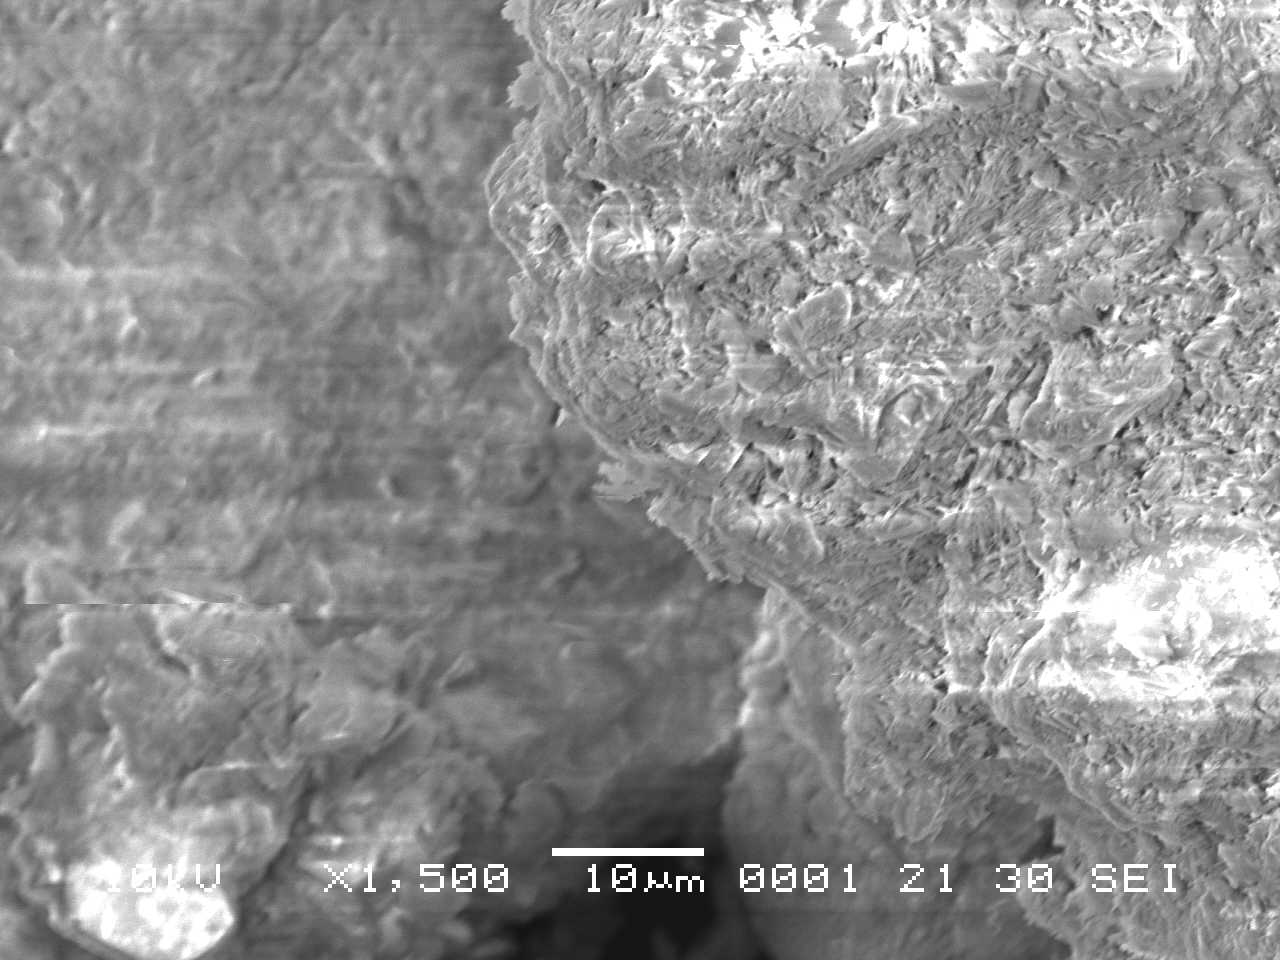
\includegraphics[width=\linewidth]{HKI_natural_azurite_x1500_2_040521}
\end{minipage}
\begin{minipage}{.45\textwidth}
  \centering
  \includegraphics[width=\linewidth]{HKI_natural_azurite_x1500_4_040521}
\end{minipage}
\caption[SEM images: Sample HKI, natural azurite]{SEM images: Sample HKI, natural azurite. Magnification: 1500x.}
\label{fig:hki_nat_az_sem_4}
\end{figure}

\begin{figure}[H]
\centering
\begin{minipage}{.45\textwidth}
  \centering
  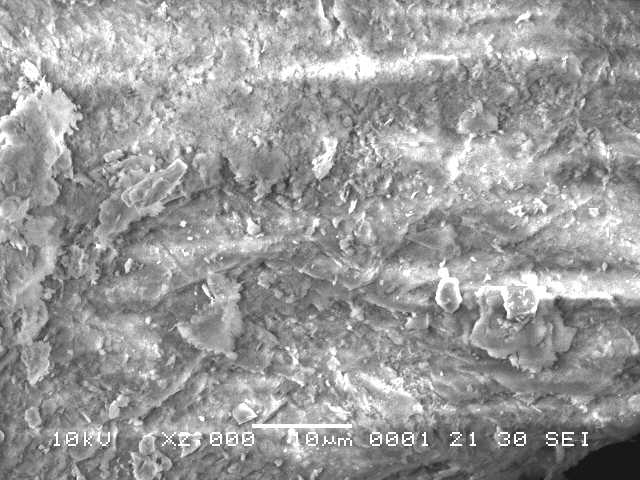
\includegraphics[width=\linewidth]{HKI_natural_azurite_x2000_1_040521}
\end{minipage}
\begin{minipage}{.45\textwidth}
  \centering
  \includegraphics[width=\linewidth]{HKI_natural_azurite_x4000_2_040521}
\end{minipage}
\caption[SEM images: Sample HKI, natural azurite]{SEM images: Sample HKI, natural azurite. Magnification: \textbf{left)} 2000x, \textbf{right)} 4000x.}
\label{fig:hki_nat_az_sem_5}
\end{figure}

\textit{Figure \ref{fig:az1_sem_2}} shows Az 1 at 750x (left) and 1500x (right). At 1500x, it is possible to observe smaller voluminous (not flat) particles on the surface of larger particles. The vast majority of pieces are irregularly shaped with choppy borders, though a few circular particles are also present.

\begin{figure}[H]
\centering
\begin{minipage}{.45\textwidth}
  \centering
  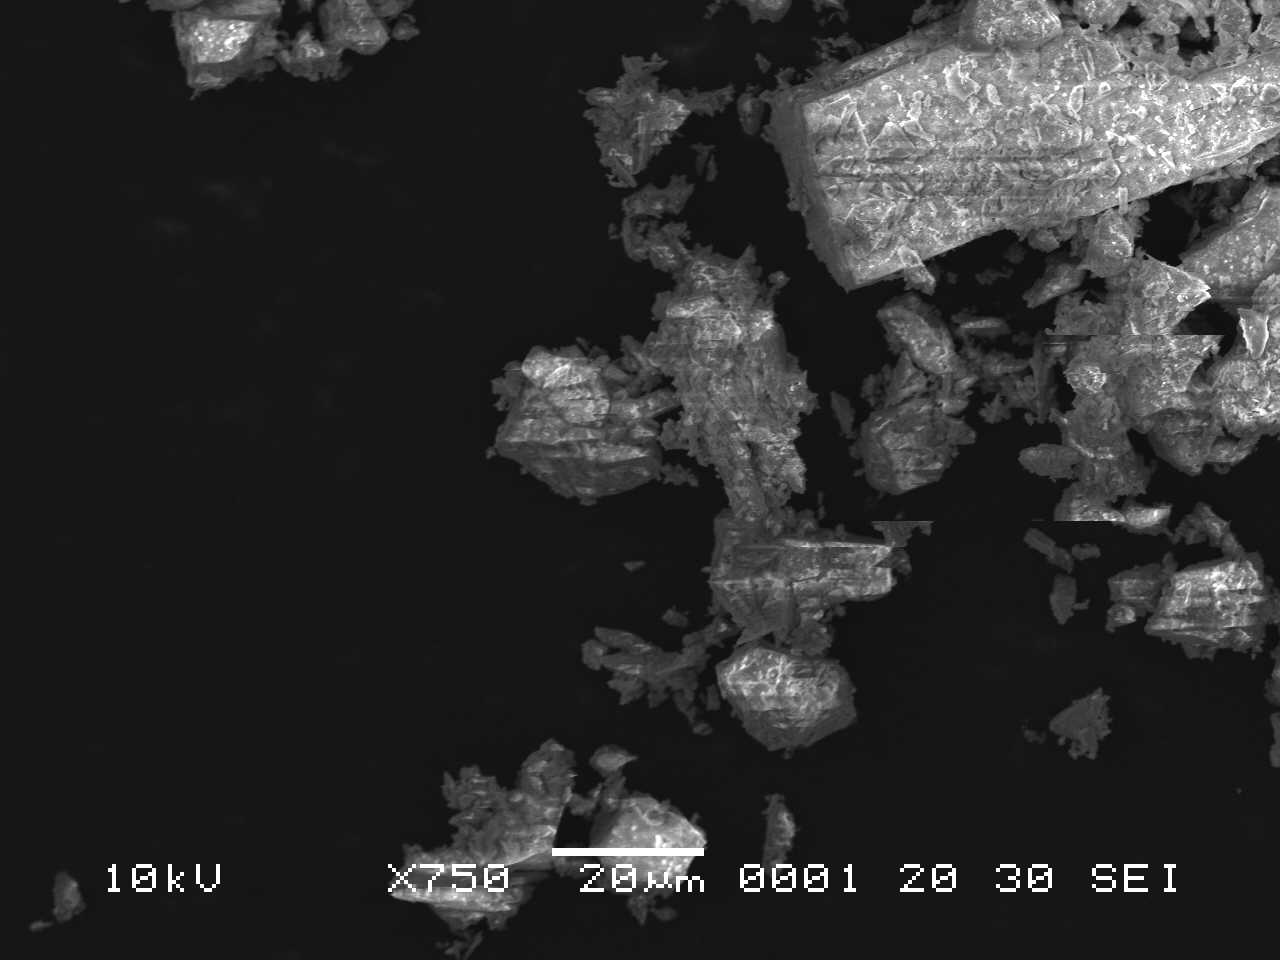
\includegraphics[width=\linewidth]{Az1_x750_6_220221}
\end{minipage}
\begin{minipage}{.45\textwidth}
  \centering
  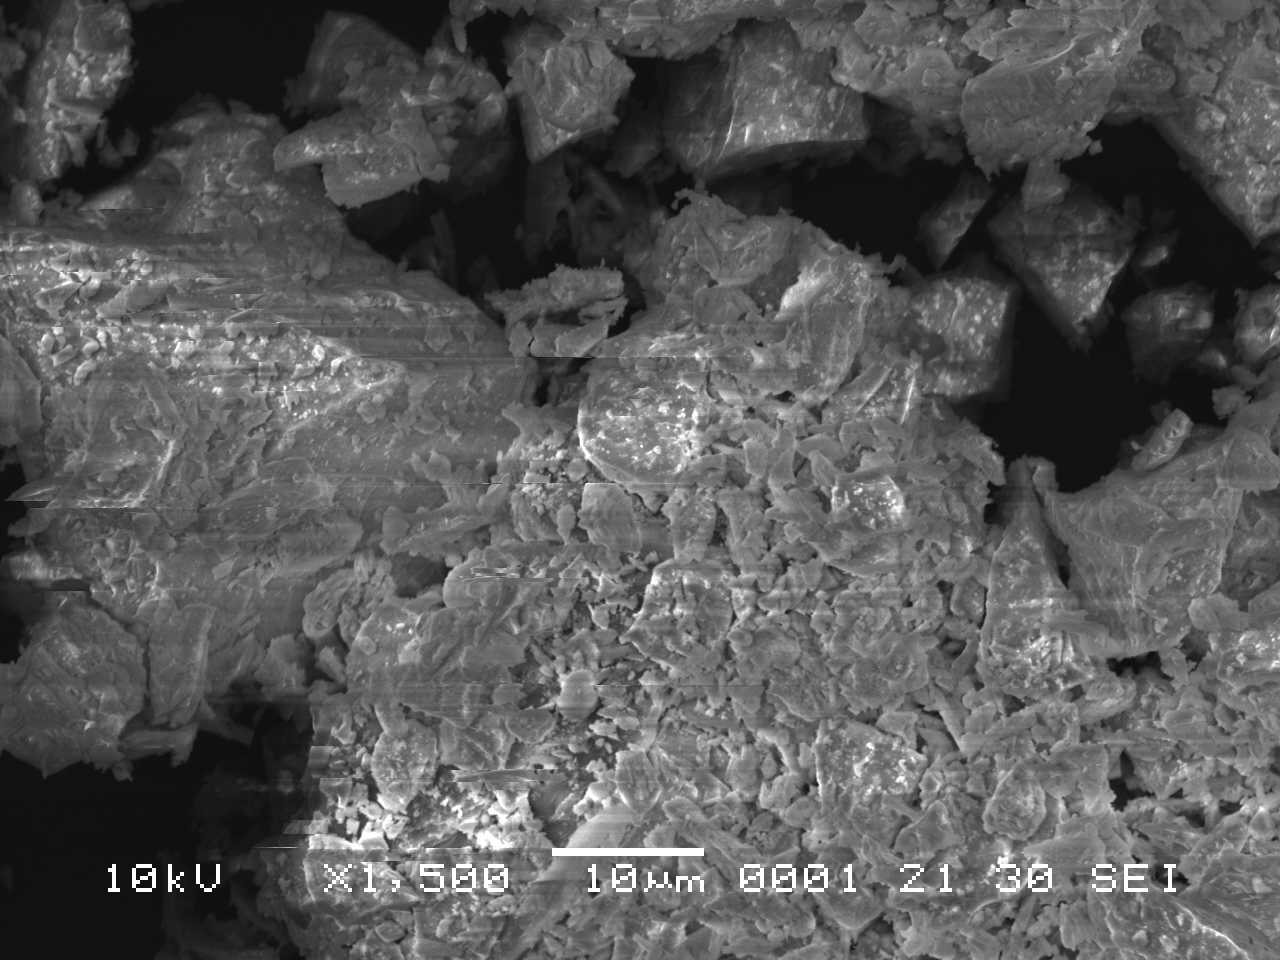
\includegraphics[width=\linewidth]{Az1_x1500_2_220221}
\end{minipage}
\caption[SEM images: Sample Az1, azurite]{SEM images: Sample Az1, azurite. Magnification: \textbf{left)} 750x, \textbf{right)} 1500x.}
\label{fig:az1_sem_2}
\end{figure}

At 750x magnification, sample Az 2 shows particles with flat sides. There is slightly more size variation than initially seen, though this is difficult to assess due to jumping of particles during charging.

\begin{figure}[H]
\centering
\begin{minipage}{.45\textwidth}
  \centering
  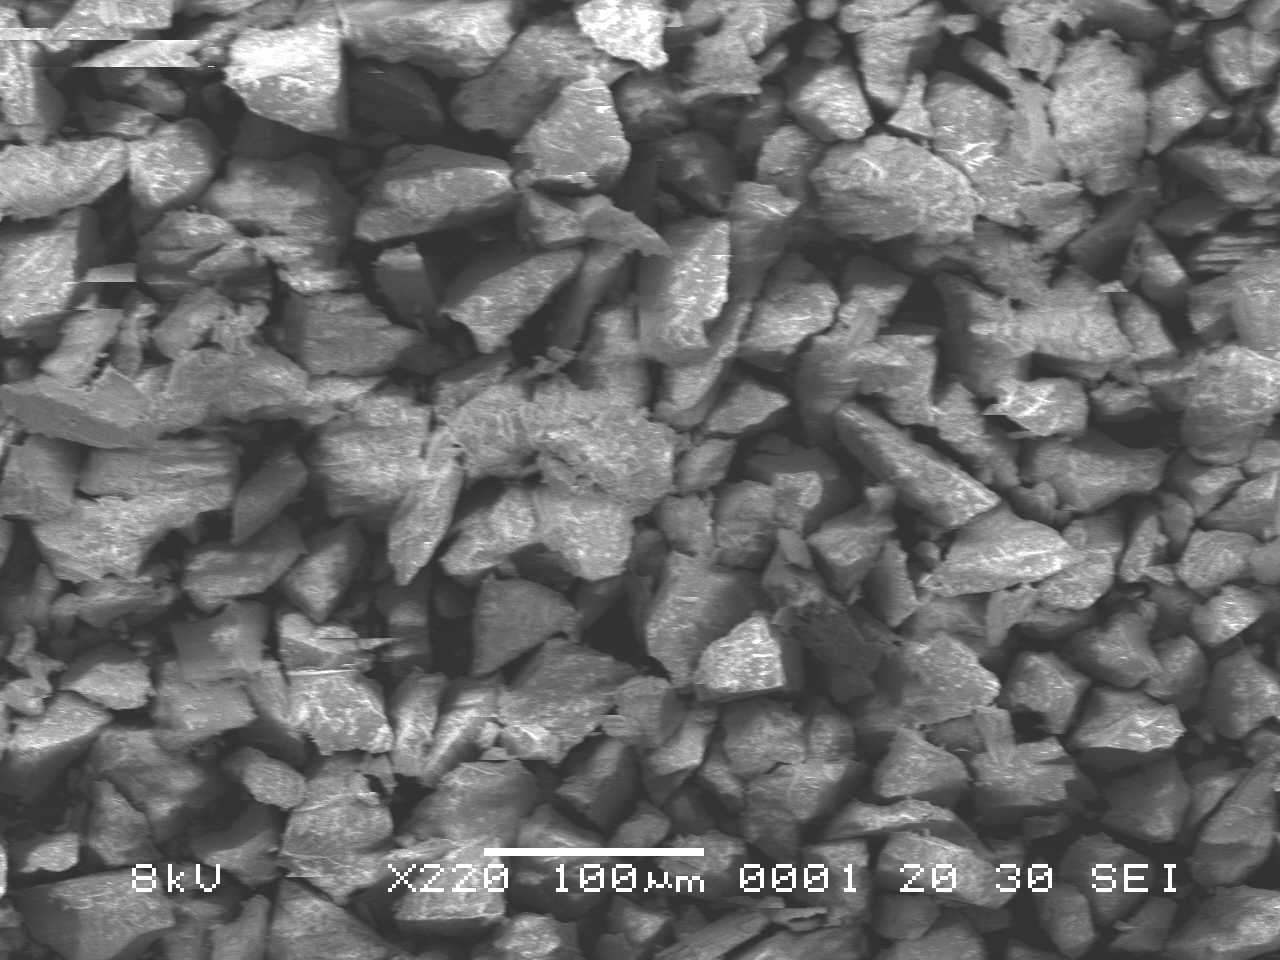
\includegraphics[width=\linewidth]{Az2_x200_2_240221}
\end{minipage}
\begin{minipage}{.45\textwidth}
  \centering
  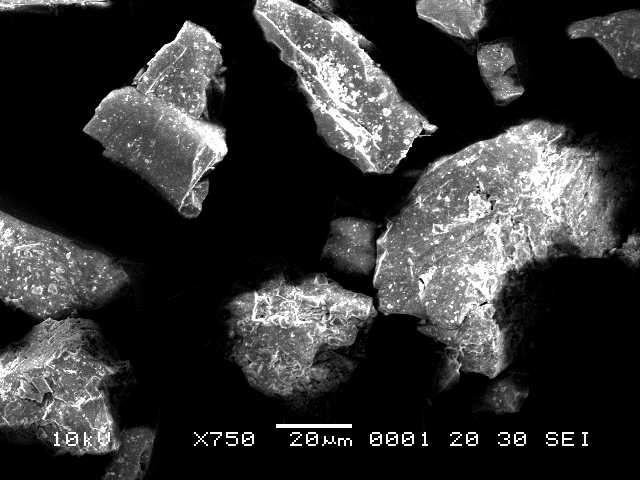
\includegraphics[width=\linewidth]{Az2_x750_1_150321}
\end{minipage}
\caption[SEM images: Sample Az2, azurite]{SEM images: Sample Az2, azurite. Magnification: \textbf{left)} 200x, \textbf{right)} 750x.}
\label{fig:az2_sem_2}
\end{figure}


At 200-250x magnification (\textit{Figure \ref{fig:azmag_sem_2}}), extremely small particles are shown in sample AzMag. The particle size is fairly homogeneous, though there is a great deal of variation in particle shape as well as a lot of texture observed.

\begin{figure}[H]
\centering
\begin{minipage}{.45\textwidth}
  \centering
  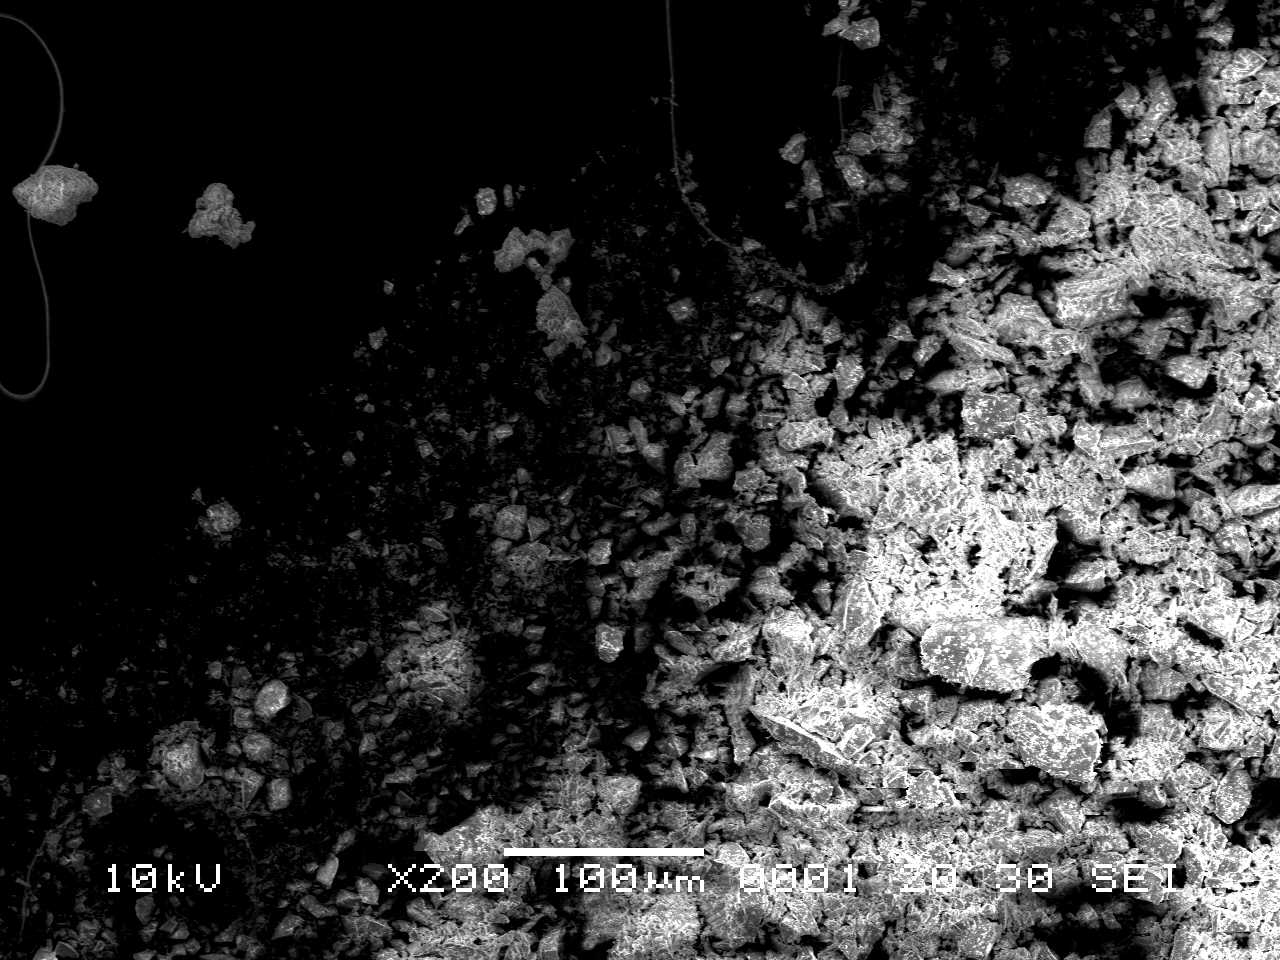
\includegraphics[width=\linewidth]{AzMag_x200_1_260221}
\end{minipage}
\begin{minipage}{.45\textwidth}
  \centering
  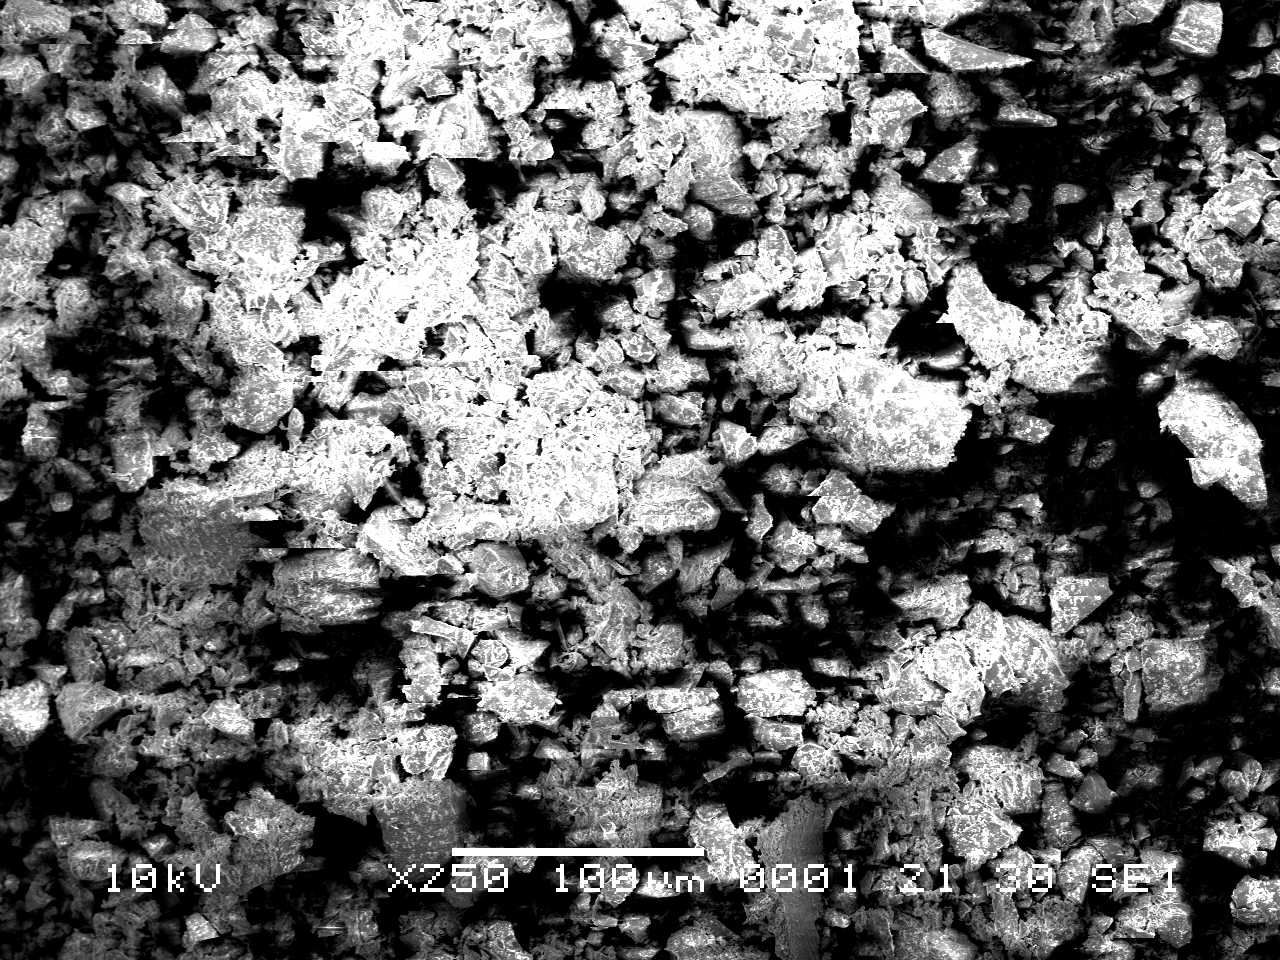
\includegraphics[width=\linewidth]{AzMag_x250_2_160321}
\end{minipage}
\caption[SEM images: Sample AzMag, azurite]{SEM images: Sample AzMag, azurite. Magnification: \textbf{left)} 200x, \textbf{right)} 250x}
\label{fig:azmag_sem_2}
\end{figure}

\begin{figure}[H]
\centering
\begin{minipage}{.45\textwidth}
  \centering
  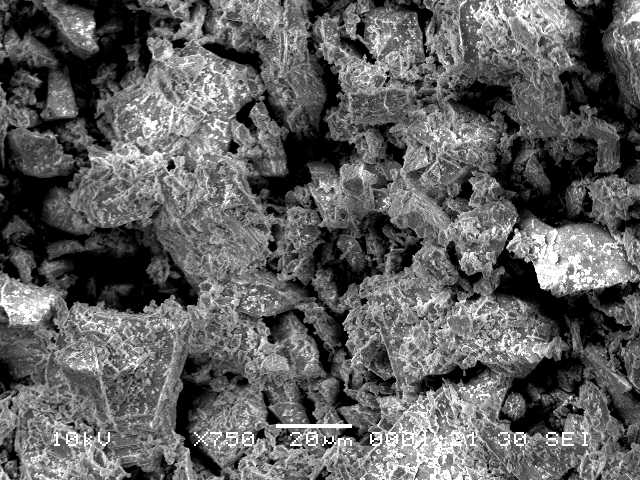
\includegraphics[width=\linewidth]{AzMag_x750_3_160321}
\end{minipage}
\begin{minipage}{.45\textwidth}
  \centering
  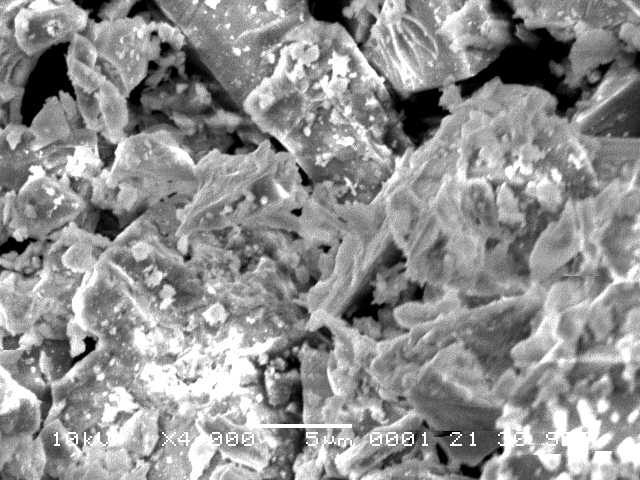
\includegraphics[width=\linewidth]{AzMag_x4000_1_160321}
\end{minipage}
\caption[SEM images: Sample AzMag, azurite]{SEM images: Sample AzMag, azurite. Magnification: \textbf{left)} 750x, \textbf{right)} 4000x.}
\label{fig:azmag_sem_3}
\end{figure}

\textit{Figure \ref{fig:azmag_sem_4}} and the left image in \textit{Figure \ref{fig:azmag_sem_5}} show the sample at 1500x magnification. Here, sample AzMag is qualitatively similar to HKI natural azurite. There are thinnner forms, though they are not quite as delicate as the needle like formations discussed previously.


\begin{figure}[H]
\centering
\begin{minipage}{.45\textwidth}
  \centering
  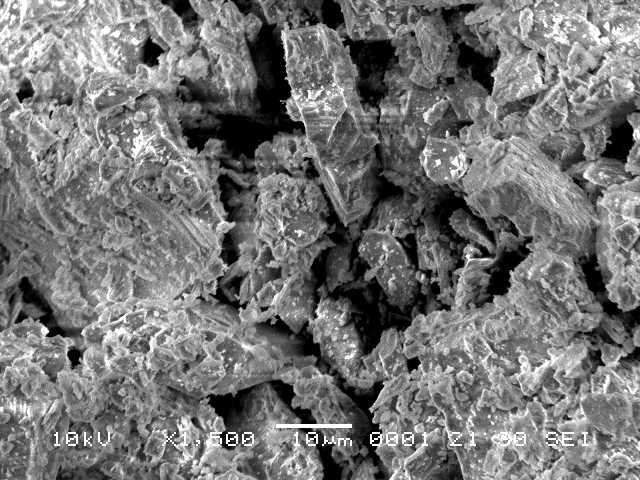
\includegraphics[width=\linewidth]{AzMag_x1500_1_160321}
\end{minipage}
\begin{minipage}{.45\textwidth}
  \centering
  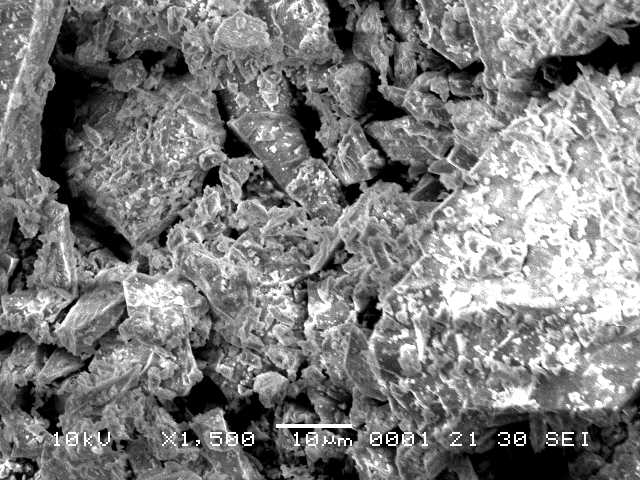
\includegraphics[width=\linewidth]{AzMag_x1500_3_160321}
\end{minipage}
\caption[SEM images: Sample AzMag, azurite]{SEM images: Sample AzMag, azurite. Magnification: 1500x}
\label{fig:azmag_sem_4}
\end{figure}

\begin{figure}[H]
\centering
\begin{minipage}{.45\textwidth}
  \centering
  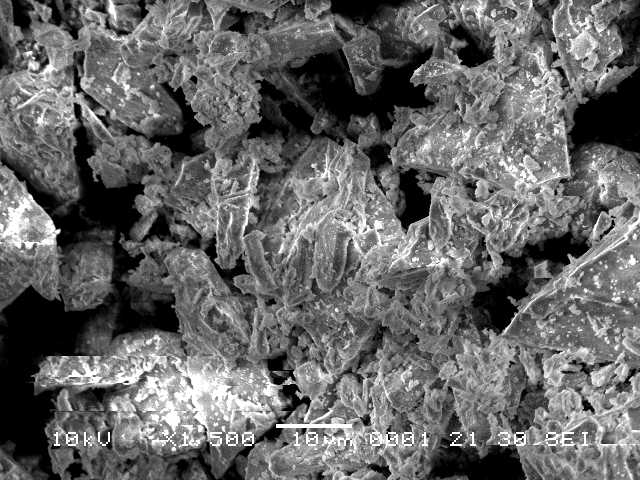
\includegraphics[width=\linewidth]{AzMag_x1500_5_160321}
\end{minipage}
\begin{minipage}{.45\textwidth}
  \centering
  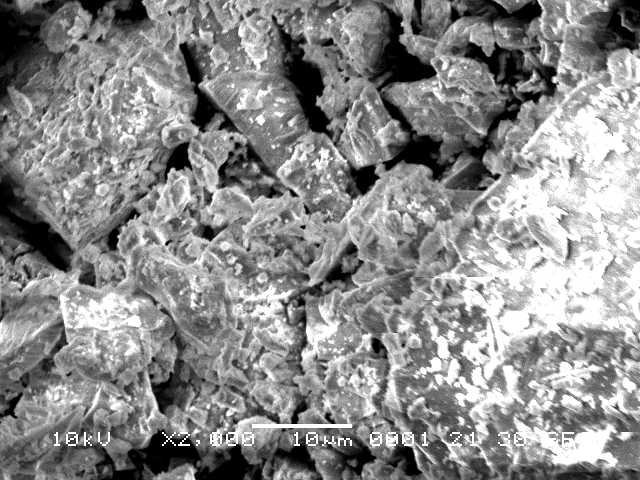
\includegraphics[width=\linewidth]{AzMag_x2000_1_160321}
\end{minipage}
\caption[SEM images: Sample AzMag, azurite]{SEM images: Sample AzMag, azurite. Magnification: \textbf{left)} 1500x, \textbf{right)} 2000x}
\label{fig:azmag_sem_5}
\end{figure}



At 250x magnification (\textit{Figure \ref{fig:azop_sem_3}}, left), small and very textured particles are observed. The size of these particles is fairly homogenous. 

\begin{figure}[H]
\centering
  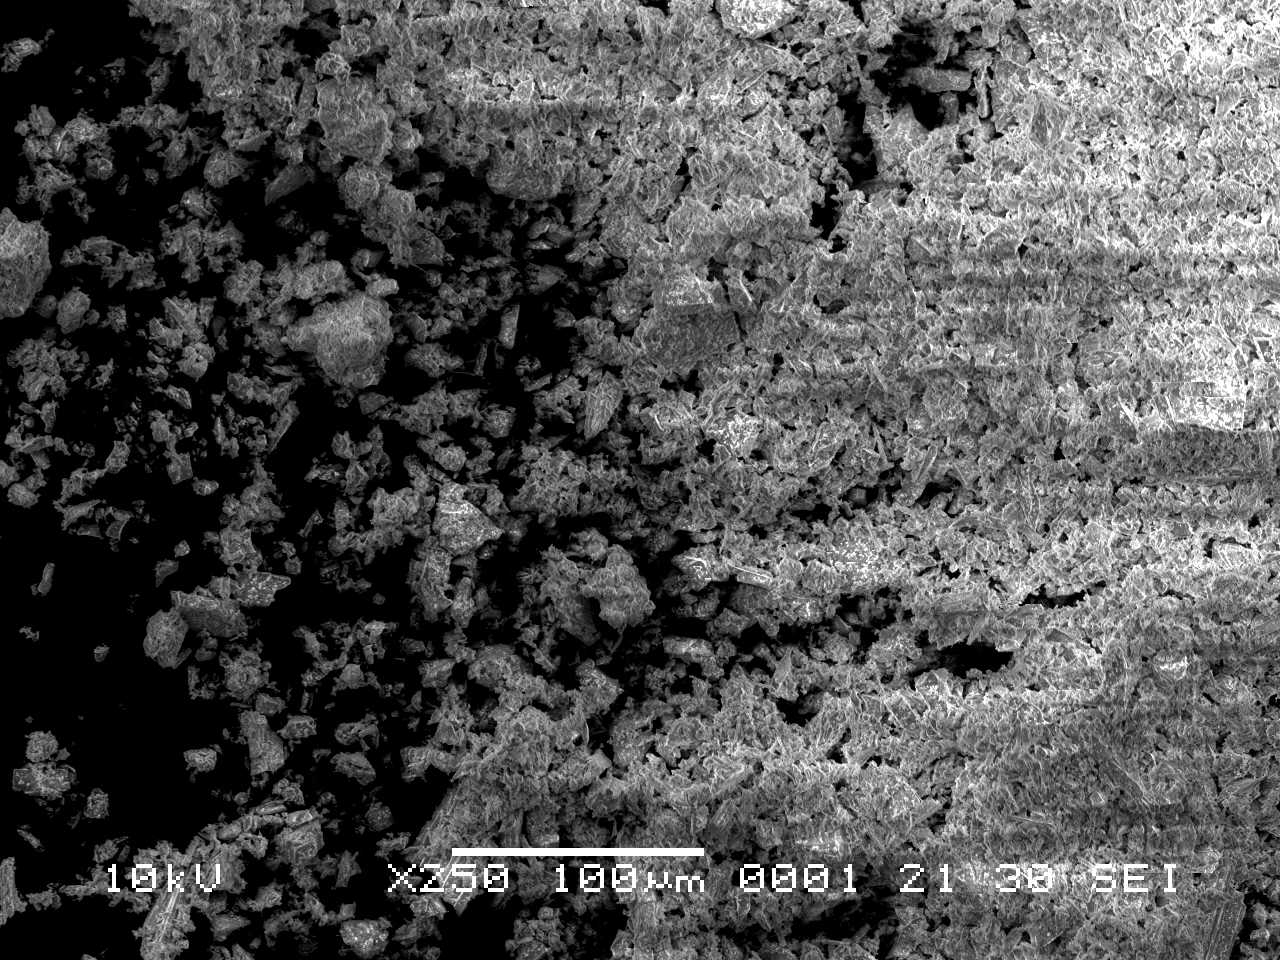
\includegraphics[width=\linewidth]{AzOp_x250_1_150321}
\caption[SEM images: Sample AzOp, azurite]{SEM images: Sample AzOp, azurite. Magnification: 250x.}
\label{fig:azop_sem_3}
\end{figure}

\begin{figure}[H]
\centering
\begin{minipage}{.45\textwidth}
  \centering
  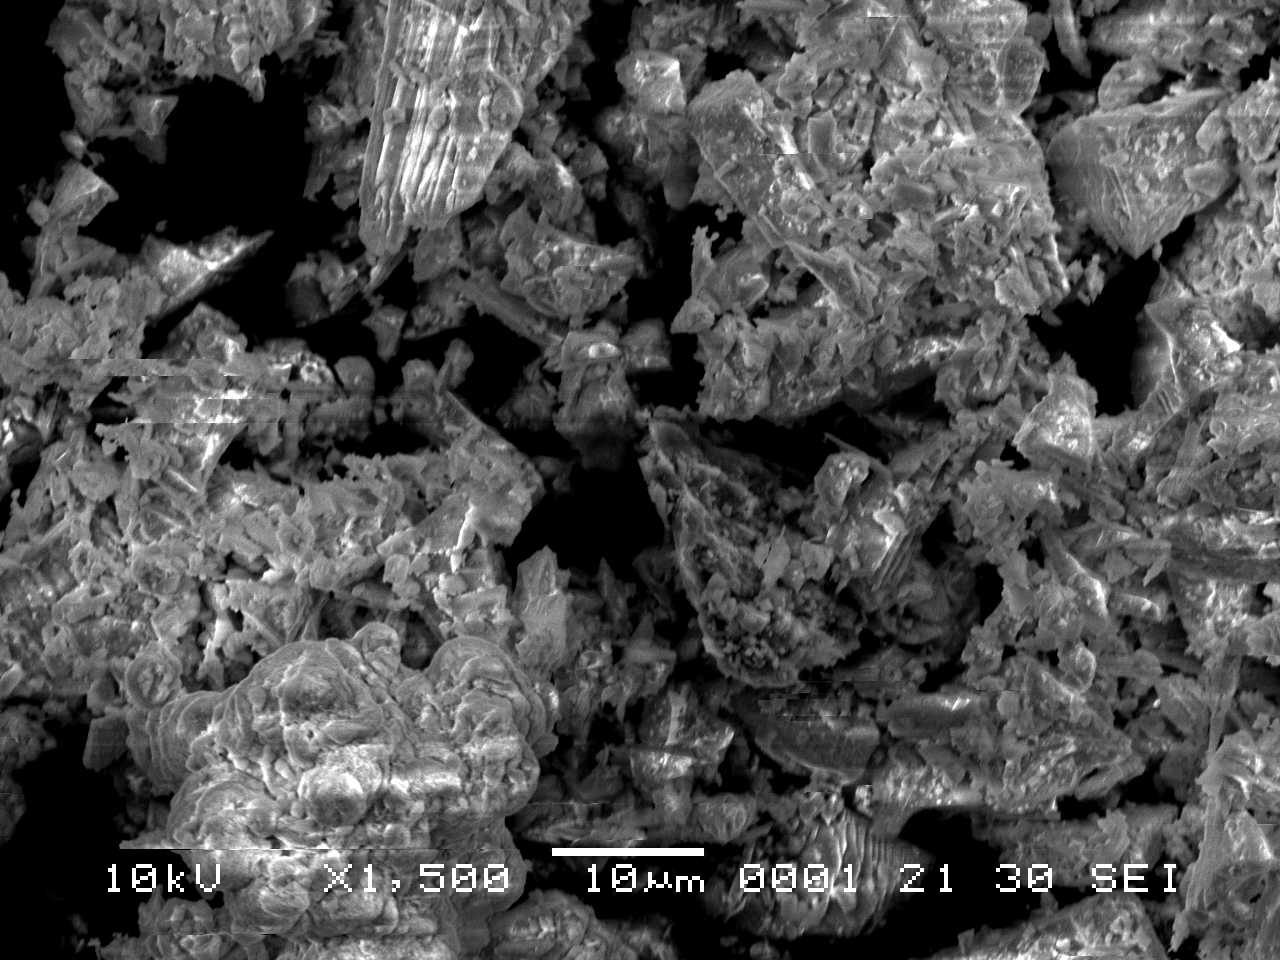
\includegraphics[width=\linewidth]{AzOp_x1500_2_150321}
\end{minipage}
\begin{minipage}{.45\textwidth}
  \centering
  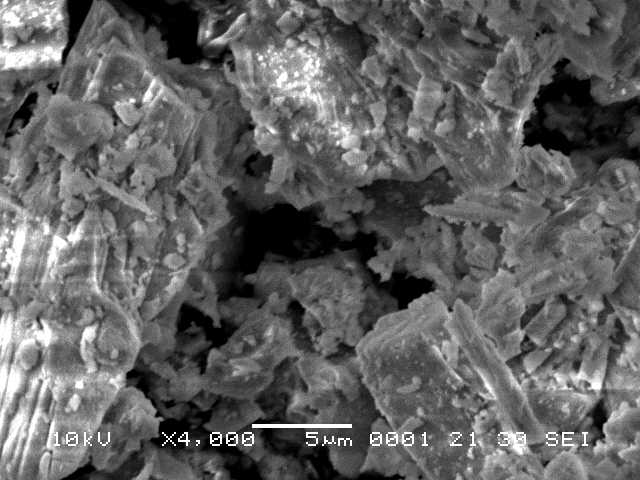
\includegraphics[width=\linewidth]{AzOp_x4000_1_150321}
\end{minipage}
\caption[SEM images: Sample AzOp, azurite]{SEM images: Sample AzOp, azurite. Magnification: \textbf{left)} 1500x, \textbf{right)} 4000x}
\label{fig:azop_sem_4}
\end{figure}


At 250x magnification (\textit{Figure \ref{fig:Fitz1_sem_2}}, left), sample Fitz 1 shows small uniform particles. These appear generally circular and far more consistent in size and shape than the samples discussed thus far. The image shown at 2500x magnification (\textit{Figure \ref{fig:Fitz1_sem_2}}, right) is of lower quality due to surface charging and jumping which made slower acquisitions unsuccessful. The faster acquisition does appear to flatten the image somewhat, which is important to consider since this makes it difficult to judge the volume of particles. There appear to be relatively flat aggregations of approximately circular particles with diameters of approximately 5 $\mu$m.


\begin{figure}[H]
\centering
\begin{minipage}{.45\textwidth}
  \centering
  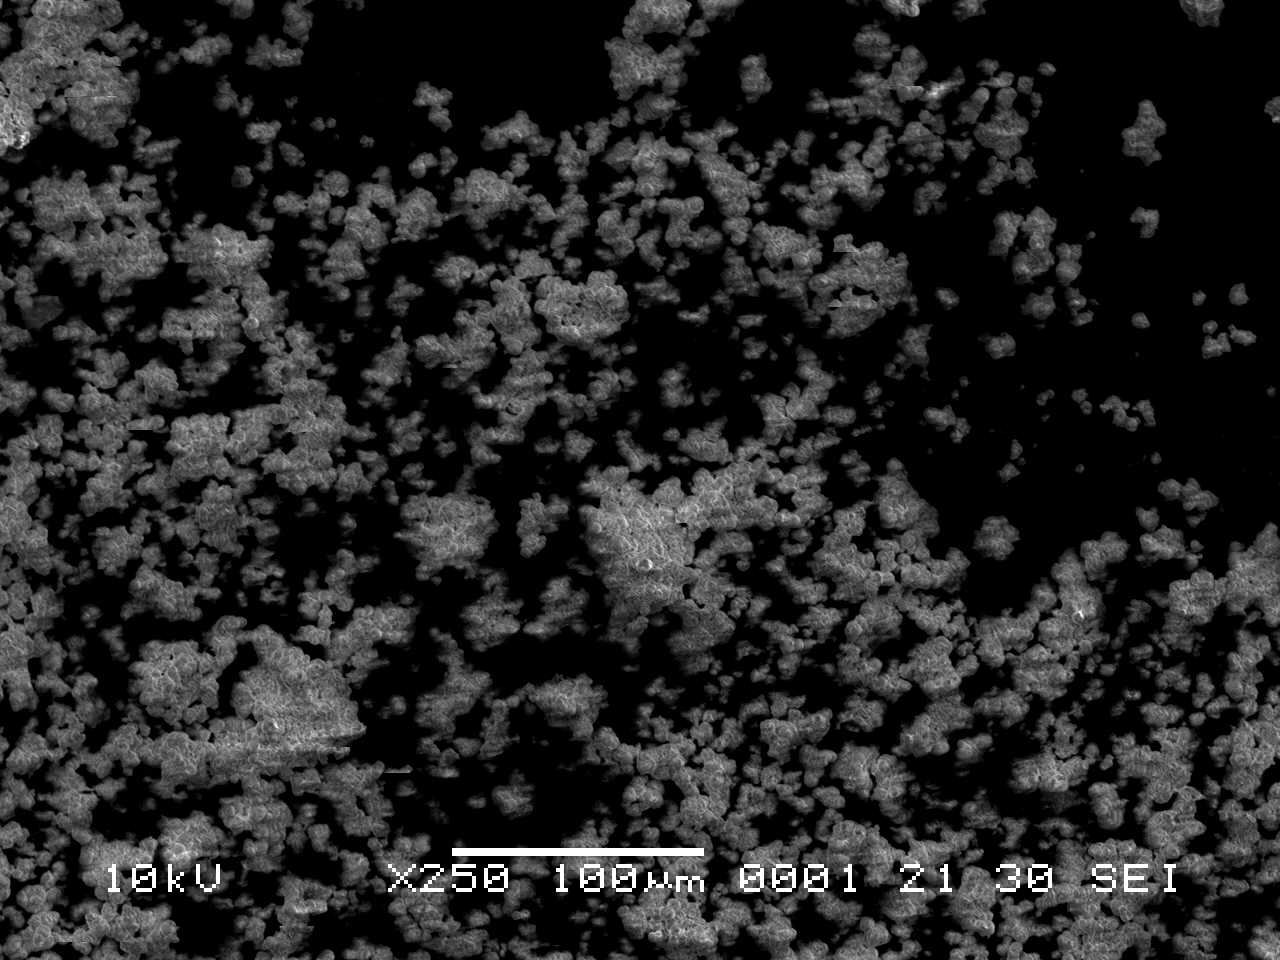
\includegraphics[width=\linewidth]{Fitz1_x250_1_030321}
\end{minipage}
\begin{minipage}{.45\textwidth}
  \centering
  \includegraphics[width=\linewidth]{Fitz1_x2500_1_030321}
\end{minipage}
\caption[SEM images: Sample Fitz1, blue verditer]{SEM images: Sample Fitz1, blue verditer. Magnification: \textbf{left)} 250x, \textbf{right)} 2500x}
\label{fig:Fitz1_sem_2}
\end{figure}



The image collected at 250x magnification (\textit{Figure \ref{fig:KE3_sem_2}}, left) showed minor issues with charging. Very small particles are present with minimal aggregation. These appear very uniform in size and slightly spherical. The approximate particle size can be approximated to 5-10 $\mu$m from the image collected at 1500x magnification (\textit{Figure \ref{fig:KE3_sem_2}}, right). The surfaces appear more porous or pocked than sample Fitz 1, but particles are more spherical and uniform than samples from natural origin. 


\begin{figure}[H]
\centering
\begin{minipage}{.45\textwidth}
  \centering
  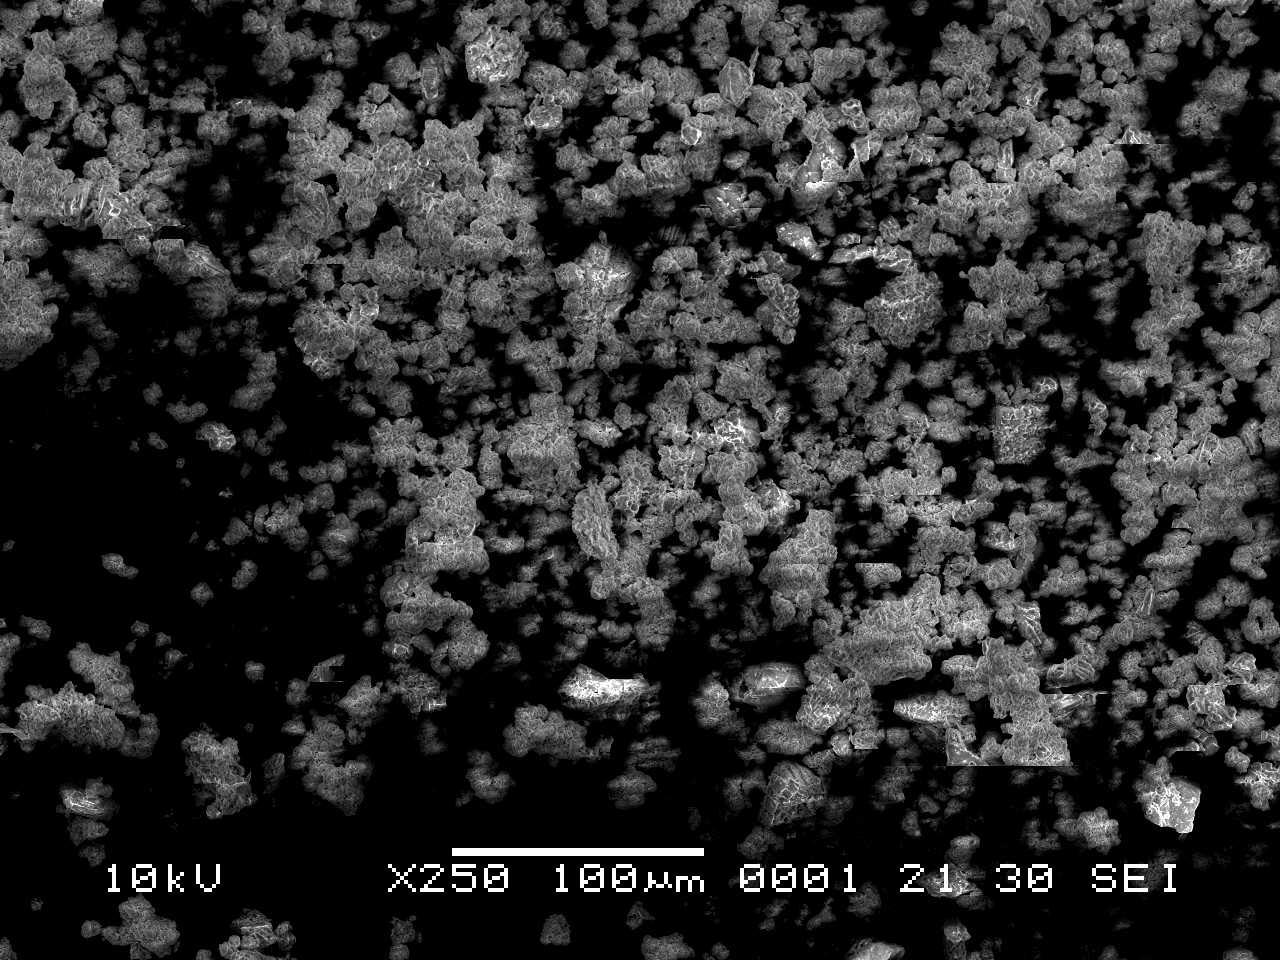
\includegraphics[width=\linewidth]{KE3_x250_1_050321}
\end{minipage}
\begin{minipage}{.45\textwidth}
  \centering
  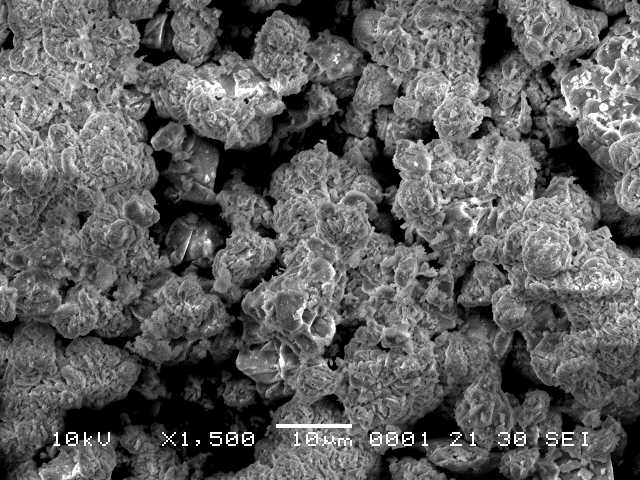
\includegraphics[width=\linewidth]{KE3_x1500_1_050321}
\end{minipage}
\caption[SEM images: Sample KE 3, light verditer bice]{SEM images: Sample KE 3, light verditer bice. Magnification: \textbf{left)} 250x, \textbf{right)} 1500x.}
\label{fig:KE3_sem_2}
\end{figure}

\textit{Figure \ref{fig:KE4_sem_2}} (right) shows sample KE 4 at 1000x magnification, where the fine structure resembling needles or feathers is very clear. These structures are not oriented in any way, and appear randomly assembled.

\begin{figure}[H]
\centering
\begin{minipage}{.45\textwidth}
  \centering
  \includegraphics[width=\linewidth]{KE4_x250_1_030321}
\end{minipage}
\begin{minipage}{.45\textwidth}
  \centering
  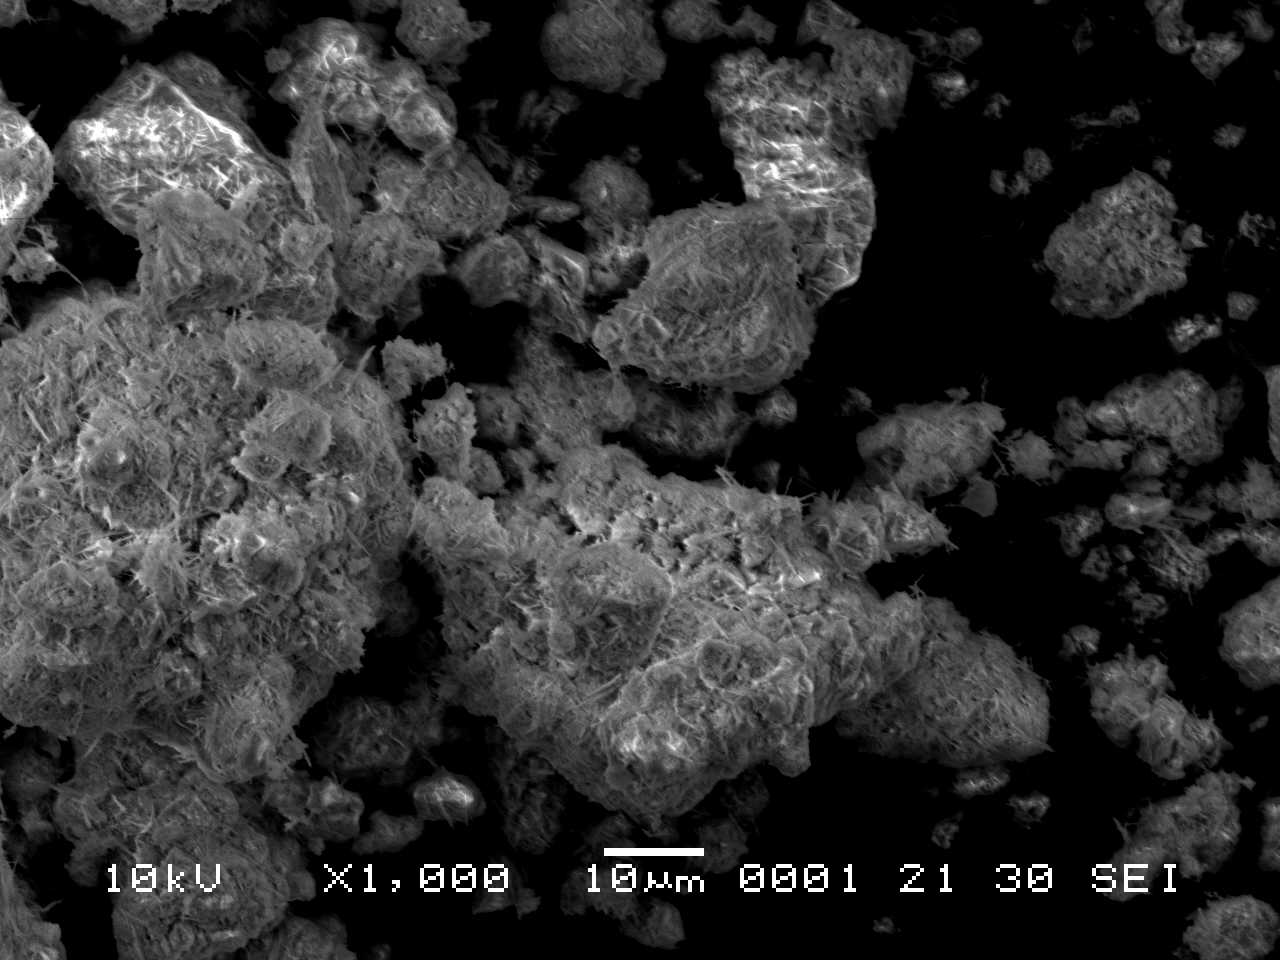
\includegraphics[width=\linewidth]{KE4_x1000_1_030321}
\end{minipage}
\caption[SEM images: Sample KE4, blue bice]{SEM images: Sample KE4, blue bice. Magnification: \textbf{left)} 250x, \textbf{right)} 1000x}
\label{fig:KE4_sem_2}
\end{figure}


\textit{Figure \ref{fig:KE5_sem_2}} (left) shows KE 5 at 250x magnification. Small circular particles of uniform size and shape are observed.

\begin{figure}[H]
\centering
\begin{minipage}{.45\textwidth}
  \centering
  \includegraphics[width=\linewidth]{KE5_x250_2_050321}
\end{minipage}
\begin{minipage}{.45\textwidth}
  \centering
  \includegraphics[width=\linewidth]{KE5_x2000_2_050321}
\end{minipage}
\caption[SEM images: Sample KE 5, blue verditer]{SEM images: Sample KE 5, blue verditer. Magnification: \textbf{left)} 250x, \textbf{right)} 2000x}
\label{fig:KE5_sem_2}
\end{figure}


\begin{comment}
Image thresholding

\begin{figure}[H]
\centering
\begin{minipage}{.45\textwidth}
  \centering
  \includegraphics[width=\linewidth]{HKI_natural_azurite_x750_1_130521}
\end{minipage}
\begin{minipage}{.45\textwidth}
  \centering
  \includegraphics[width=\linewidth]{HKI_natural_azurite_x750_1_130521-2_BW}
\end{minipage}
\caption[Particle size analysis: Sample HKI natural azurite]{Particle size analysis: Sample HKI natural azurite. \textbf{Left)} original SEM image, \textbf{Right)} thresholded binary image.}
\label{fig:imageJ_hki}
\end{figure}
\end{comment}

At low magnification (200-250x) as shown in \textit{Figure \ref{fig:Ma1_sem_3}}, sample Ma 1 appears extremely powdery and fine. The size and shape of particles are extremely irregular in both size and shape. At 1500x magnification (\textit{Figure \ref{fig:Ma1_sem_4}}), the texture of surfaces of the large (approx. 20 $\mu$m) aggregates is observed. It consists of particles of less than 5 $\mu$m across. 

\begin{figure}[H]
\centering
\begin{minipage}{.45\textwidth}
  \centering
  \includegraphics[width=\linewidth]{Ma1_x200_1_240221}
\end{minipage}
\begin{minipage}{.45\textwidth}
  \centering
  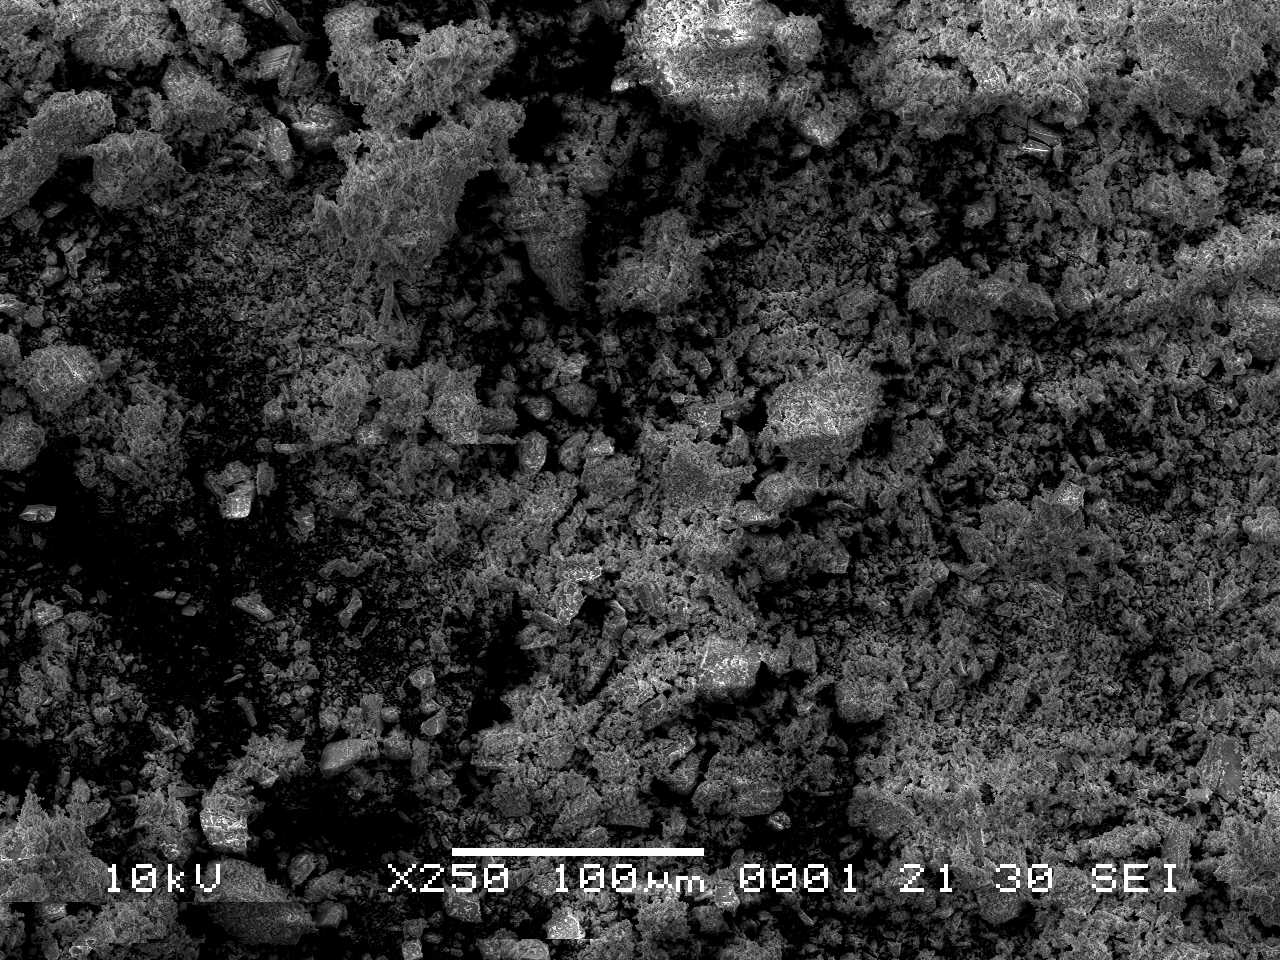
\includegraphics[width=\linewidth]{Ma1_x250_2_160321}
\end{minipage}
\caption[SEM images: Sample Ma 1, malachite]{SEM images: Sample Ma 1, malachite. Magnification: \textbf{left)} 200x, \textbf{right)} 250x}
\label{fig:Ma1_sem_3}
\end{figure}

\begin{figure}[H]
\centering
  \includegraphics[width=0.45\linewidth]{Ma1_x1500_2_160321}
\caption[SEM images: Sample Ma 1, malachite]{SEM images: Sample Ma 1, malachite. Magnification: 1500x.}
\label{fig:Ma1_sem_4}
\end{figure}

\begin{figure}[H]
\centering
\begin{minipage}{.45\textwidth}
  \centering
  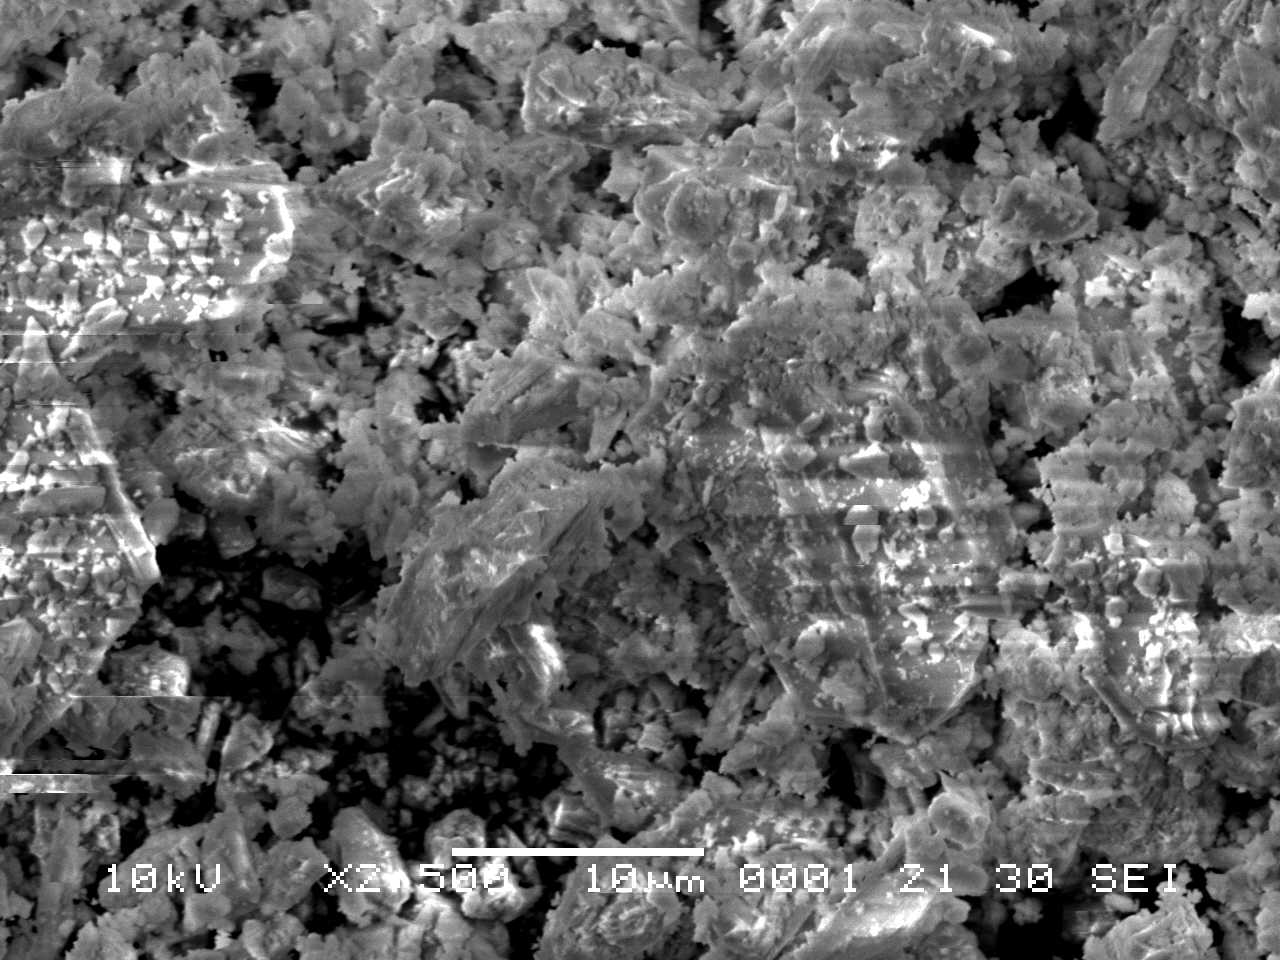
\includegraphics[width=\linewidth]{Ma1_x2500_2_160321}
\end{minipage}
\begin{minipage}{.45\textwidth}
  \centering
  \includegraphics[width=\linewidth]{Ma1_x4000_1_160321}
\end{minipage}
\caption[SEM images: Sample Ma 1, malachite]{SEM images: Sample Ma 1, malachite. Magnification: \textbf{left)} 2500x, \textbf{right)} 4000x.}
\label{fig:Ma1_sem_5}
\end{figure}



At 250x magnification (\textit{Figure \ref{fig:KE2_sem_2}} left), sample KE 2 sample appears fairly uniform in size and shape. It is very finely ground or naturally consists of small crystals and aggregates. It is possible to estimate the particle size at approximately 7-10 $\mu$m in the image at 1500x magnification.

\begin{figure}[H]
\centering
\begin{minipage}{.45\textwidth}
  \centering
  \includegraphics[width=\linewidth]{KE2_250_1_040321}
\end{minipage}
\begin{minipage}{.45\textwidth}
  \centering
  \includegraphics[width=\linewidth]{KE2_x1500_040321}
\end{minipage}
\caption[SEM images: Sample KE 2, green verditer]{SEM images: Sample KE 2, green verditer. Magnification: \textbf{left)} 250x, \textbf{right)} 1500x.}
\label{fig:KE2_sem_2}
\end{figure}



\begin{figure}[H]
\centering
\begin{minipage}{.45\textwidth}
  \centering
  \includegraphics[width=\linewidth]{hki_xsection_BES_LV_x550_40spot_250621}
\end{minipage}
\begin{minipage}{.45\textwidth}
  \centering
  \includegraphics[width=\linewidth]{hki_xsection_BES_LV_x550_58spot_240621}
\end{minipage}
\caption[SEM images: Historical cross section, azurite and blue verditer]{SEM images: Historical cross section, azurite and blue verditer, JEOL SEM. Magnification: 550x}
\label{fig:xsection_jeol_3}
\end{figure}

\begin{figure}[H]
\centering
  \includegraphics[width=0.45\linewidth]{hki_xsection_BES_LV_x750_3_58spot_240621}
\caption[SEM images: Historical cross section, azurite and blue verditer]{SEM images: Historical cross section, azurite and blue verditer, JEOL SEM. Magnification: 750x}
\label{fig:xsection_jeol_4}
\end{figure}

\begin{figure}[H]
\centering
\begin{minipage}{.45\textwidth}
  \centering
  \includegraphics[width=\linewidth]{hki_xsection_BES_LV_x750_58spot_240621}
\end{minipage}
\begin{minipage}{.45\textwidth}
  \centering
  \includegraphics[width=\linewidth]{hki_xsection_x750_2_250621}
\end{minipage}
\caption[SEM images: Historical cross section, azurite and blue verditer]{SEM images: Historical cross section, azurite and blue verditer, JEOL SEM. Magnification: 750x. Right image is collected using the secondary electron (SE) detector.}
\label{fig:xsection_jeol_5}
\end{figure}


\begin{figure}[H]
\centering
\begin{minipage}{.45\textwidth}
  \centering
  \includegraphics[width=\linewidth]{hki_xsection_BES_LV_x1500_40spot_250621}
\end{minipage}
\begin{minipage}{.45\textwidth}
  \centering
  \includegraphics[width=\linewidth]{hki_xsection_BES_LV_x1500_2_40spot_250621}
\end{minipage}
\caption[SEM images: Historical cross section, azurite and blue verditer]{SEM images: Historical cross section, azurite and blue verditer, JEOL SEM. Magnification: 1500x}
\label{fig:xsection_jeol_6}
\end{figure}

\begin{figure}[H]
\centering
\begin{minipage}{.45\textwidth}
  \centering
  \includegraphics[width=\linewidth]{hki_xsection_BES_LV_x2300_2_40spot_250621}
\end{minipage}
\begin{minipage}{.45\textwidth}
  \centering
  \includegraphics[width=\linewidth]{hki_xsection_BES_LV_x2300_40spot_250621}
\end{minipage}
\caption[SEM images: Historical cross section, azurite and blue verditer]{SEM images: Historical cross section, azurite and blue verditer, JEOL SEM. Magnification: 2300x}
\label{fig:xsection_jeol_7}
\end{figure}

\begin{figure}[H]
\centering
  \includegraphics[width=0.45\linewidth]{hki_xsection_BES_LV_x2500_40spot_250621}
\caption[SEM images: Historical cross section, azurite and blue verditer]{SEM images: Historical cross section, azurite and blue verditer, JEOL SEM. Magnification: 2500x}
\label{fig:xsection_jeol_8}
\end{figure}


\begin{figure}[H]
\centering
  \includegraphics[width=0.9\linewidth]{hki_cross_section_img_290621_01}
\caption[SEM images: Historical cross section, azurite and blue verditer]{SEM images: Historical cross section, azurite and blue verditer, TESCAN SEM. Magnification: 1000x}
\label{fig:xsection_dept_3}
\end{figure}

\begin{figure}[H]
\centering
  \includegraphics[width=0.9\linewidth]{hki_cross_section_img_290621_04}
\caption[SEM images: Historical cross section, azurite and blue verditer]{SEM images: Historical cross section, azurite and blue verditer, TESCAN SEM. Magnification: 1500x}
\label{fig:xsection_dept_4}
\end{figure}


\begin{figure}[H]
\centering
  \includegraphics[width=0.9\linewidth]{hki_cross_section_img_290621_08}
\caption[SEM images: Historical cross section, azurite and blue verditer]{SEM images: Historical cross section, azurite and blue verditer, TESCAN SEM. Magnification: 2000x}
\label{fig:xsection_dept_5}
\end{figure}

\begin{figure}[H]
\centering
  \includegraphics[width=0.9\linewidth]{hki_cross_section_img_290621_03}
\caption[SEM images: Historical cross section, azurite and blue verditer]{SEM images: Historical cross section, azurite and blue verditer, TESCAN SEM. Magnification: 3500x}
\label{fig:xsection_dept_6}
\end{figure}

\begin{figure}[H]
\centering
  \includegraphics[width=0.9\linewidth]{hki_cross_section_img_290621_05}
\caption[SEM images: Historical cross section, azurite and blue verditer]{SEM images: Historical cross section, azurite and blue verditer, TESCAN SEM. Magnification: 5500x}
\label{fig:xsection_dept_7}
\end{figure}

\begin{figure}[H]
\centering
  \includegraphics[width=0.9\linewidth]{hki_cross_section_img_290621_10}
\caption[SEM images: Historical cross section, azurite and blue verditer]{SEM images: Historical cross section, azurite and blue verditer, TESCAN SEM. Magnification: 5500x}
\label{fig:xsection_dept_8}
\end{figure}



\section{EDS point spectrum data}

This data is presented in table format in Chapter 3.

\subsection{Azurite and blue verditer}

\begin{figure}[H]
\centering
\begin{minipage}{.45\textwidth}
  \centering
  \includegraphics[width=\linewidth]{HKI_nat_az_EDS_spectrum1_050521_spectrumimage}
\end{minipage}
\begin{minipage}{.45\textwidth}
  \centering
  \includegraphics[width=\linewidth]{HKI_nat_az_EDS_spectrum1_050521_semimage}
\end{minipage}
\caption[EDS point spectrum data: HKI natural azurite, sample 1]{EDS point spectrum data: HKI natural azurite, sample 1}
\label{fig:hki_point_eds_1}
\end{figure}

\begin{figure}[H]
\centering
\begin{minipage}{.45\textwidth}
  \centering
  \includegraphics[width=\linewidth]{HKI_nat_az_EDS_spectrum2_050521_spectrumimage}
\end{minipage}
\begin{minipage}{.45\textwidth}
  \centering
  \includegraphics[width=\linewidth]{HKI_nat_az_EDS_spectrum2_050521_semimage}
\end{minipage}
\caption[EDS point spectrum data: HKI natural azurite, sample 2]{EDS point spectrum data: HKI natural azurite, sample 2}
\label{fig:hki_point_eds_2}
\end{figure}

\begin{figure}[H]
\centering
\begin{minipage}{.45\textwidth}
  \centering
  \includegraphics[width=\linewidth]{HKI_nat_az_EDS_spectrum3_050521_spectrumimage}
\end{minipage}
\begin{minipage}{.45\textwidth}
  \centering
  \includegraphics[width=\linewidth]{HKI_nat_az_EDS_spectrum3_050521_semimage}
\end{minipage}
\caption[EDS point spectrum data: HKI natural azurite, sample 3]{EDS point spectrum data: HKI natural azurite, sample 3}
\label{fig:hki_point_eds_3}
\end{figure}

\begin{figure}[H]
\centering
\begin{minipage}{.45\textwidth}
  \centering
  \includegraphics[width=\linewidth]{HKI_nat_az_EDS_spectrum4_050521_spectrumimage}
\end{minipage}
\begin{minipage}{.45\textwidth}
  \centering
  \includegraphics[width=\linewidth]{HKI_nat_az_EDS_spectrum4_050521_semimage}
\end{minipage}
\caption[EDS point spectrum data: HKI natural azurite, sample 4]{EDS point spectrum data: HKI natural azurite, sample 4}
\label{fig:hki_point_eds_4}
\end{figure}

\begin{figure}[H]
\centering
\begin{minipage}{.45\textwidth}
  \centering
  \includegraphics[width=\linewidth]{HKI_nat_az_EDS_site2_spectrum1_050521_spectrumimage}
\end{minipage}
\begin{minipage}{.45\textwidth}
  \centering
  \includegraphics[width=\linewidth]{HKI_nat_az_EDS_site2_spectrum1_050521_semimage}
\end{minipage}
\caption[EDS point spectrum data: HKI natural azurite, sample 5]{EDS point spectrum data: HKI natural azurite, sample 5}
\label{fig:hki_point_eds_5}
\end{figure}

\begin{figure}[H]
\centering
\begin{minipage}{.45\textwidth}
  \centering
  \includegraphics[width=\linewidth]{HKI_nat_az_EDS_site2_spectrum2_050521_spectrumimage}
\end{minipage}
\begin{minipage}{.45\textwidth}
  \centering
  \includegraphics[width=\linewidth]{HKI_nat_az_EDS_site2_spectrum2_050521_semimage}
\end{minipage}
\caption[EDS point spectrum data: HKI natural azurite, sample 6]{EDS point spectrum data: HKI natural azurite, sample 6}
\label{fig:hki_point_eds_6}
\end{figure}

\begin{figure}[H]
\centering
\begin{minipage}{.45\textwidth}
  \centering
  \includegraphics[width=\linewidth]{HKI_nat_az_EDS_site3_spectrum1_060521_spectrumimage}
\end{minipage}
\begin{minipage}{.45\textwidth}
  \centering
  \includegraphics[width=\linewidth]{HKI_nat_az_EDS_site3_spectrum2_060521_semimage}
\end{minipage}
\caption[EDS point spectrum data: HKI natural azurite, sample 7]{EDS point spectrum data: HKI natural azurite, sample 7}
\label{fig:hki_point_eds_7}
\end{figure}

\begin{figure}[H]
\centering
\begin{minipage}{.45\textwidth}
  \centering
  \includegraphics[width=\linewidth]{HKI_nat_az_EDS_site3_spectrum2_060521_spectrumimage}
\end{minipage}
\begin{minipage}{.45\textwidth}
  \centering
  \includegraphics[width=\linewidth]{HKI_nat_az_EDS_site3_spectrum2_060521_semimage}
\end{minipage}
\caption[EDS point spectrum data: HKI natural azurite, sample 8]{EDS point spectrum data: HKI natural azurite, sample 8}
\label{fig:hki_point_eds_8}
\end{figure}




\begin{figure}[H]
\centering
\begin{minipage}{.45\textwidth}
  \centering
  \includegraphics[width=\linewidth]{Az1_EDS_1_240221_spectrumimage}
\end{minipage}
\begin{minipage}{.45\textwidth}
  \centering
  \includegraphics[width=\linewidth]{Az1_EDS_1_240221_semimage}
\end{minipage}
\caption[EDS point spectrum data: Az 1, sample 1]{EDS point spectrum data: Az 1, sample 1}
\label{fig:az1_point_eds_1}
\end{figure}

\begin{figure}[H]
\centering
\begin{minipage}{.45\textwidth}
  \centering
  \includegraphics[width=\linewidth]{Az1_EDS_2_250221_spectrumimage}
\end{minipage}
\begin{minipage}{.45\textwidth}
  \centering
  \includegraphics[width=\linewidth]{Az1_EDS_2_250221_semimage}
\end{minipage}
\caption[EDS point spectrum data: Az 1, sample 2]{EDS point spectrum data: Az 1, sample 2}
\label{fig:az1_point_eds_2}
\end{figure}

\begin{figure}[H]
\centering
\begin{minipage}{.45\textwidth}
  \centering
  \includegraphics[width=\linewidth]{Az1_EDS_3_250221_spectrumimage}
\end{minipage}
\begin{minipage}{.45\textwidth}
  \centering
  \includegraphics[width=\linewidth]{Az1_EDS_3_250221_semimage}
\end{minipage}
\caption[EDS point spectrum data: Az 1, sample 3]{EDS point spectrum data: Az 1, sample 3}
\label{fig:az1_point_eds_3}
\end{figure}

\begin{figure}[H]
\centering
\begin{minipage}{.45\textwidth}
  \centering
  \includegraphics[width=\linewidth]{Az1_EDS_4_15keV_250221_spectrumimage}
\end{minipage}
\begin{minipage}{.45\textwidth}
  \centering
  \includegraphics[width=\linewidth]{Az1_EDS_4_15keV_250221_semimage}
\end{minipage}
\caption[EDS point spectrum data: Az 1, sample 4]{EDS point spectrum data: Az 1, sample 4. Accelerating voltage: 15 keV.}
\label{fig:az1_point_eds_4}
\end{figure}

\begin{figure}[H]
\centering
\begin{minipage}{.45\textwidth}
  \centering
  \includegraphics[width=\linewidth]{Az1_EDS_5_250221_spectrumimage}
\end{minipage}
\begin{minipage}{.45\textwidth}
  \centering
  \includegraphics[width=\linewidth]{Az1_EDS_5_250221_semimage}
\end{minipage}
\caption[EDS point spectrum data: Az 1, sample 5]{EDS point spectrum data: Az 1, sample 5}
\label{fig:az1_point_eds_5}
\end{figure}

\begin{figure}[H]
\centering
\begin{minipage}{.45\textwidth}
  \centering
  \includegraphics[width=\linewidth]{Az1_EDS_6_250221_spectrumimage}
\end{minipage}
\begin{minipage}{.45\textwidth}
  \centering
  \includegraphics[width=\linewidth]{Az1_EDS_6_250221_semimage}
\end{minipage}
\caption[EDS point spectrum data: Az 1, sample 6]{EDS point spectrum data: Az 1, sample 6}
\label{fig:az1_point_eds_6}
\end{figure}



\begin{figure}[H]
\centering
\begin{minipage}{.45\textwidth}
  \centering
  \includegraphics[width=\linewidth]{Az2_EDS_1_250221_spectrumimage}
\end{minipage}
\begin{minipage}{.45\textwidth}
  \centering
  \includegraphics[width=\linewidth]{Az2_EDS_1_250221_semimage}
\end{minipage}
\caption[EDS point spectrum data: Az 2, sample 1]{EDS point spectrum data: Az 2, sample 1}
\label{fig:az2_point_eds_1}
\end{figure}

\begin{figure}[H]
\centering
\begin{minipage}{.45\textwidth}
  \centering
  \includegraphics[width=\linewidth]{az2_EDS_2_250221_spectrumimage}
\end{minipage}
\begin{minipage}{.45\textwidth}
  \centering
  \includegraphics[width=\linewidth]{az2_EDS_2_250221_semimage}
\end{minipage}
\caption[EDS point spectrum data: Az 2, sample 2]{EDS point spectrum data: Az 2, sample 2}
\label{fig:az2_point_eds_2}
\end{figure}


\begin{figure}[H]
\centering
\begin{minipage}{.45\textwidth}
  \centering
  \includegraphics[width=\linewidth]{AzMag_EDS_1_260220_spectrumimage}
\end{minipage}
\begin{minipage}{.45\textwidth}
  \centering
  \includegraphics[width=\linewidth]{AzMag_EDS_1_260220_semimage}
\end{minipage}
\caption[EDS point spectrum data: AzMag, sample 1]{EDS point spectrum data: AzMag, sample 1}
\label{fig:azmag_point_eds_1}
\end{figure}

\begin{figure}[H]
\centering
\begin{minipage}{.45\textwidth}
  \centering
  \includegraphics[width=\linewidth]{AzMag_EDS_2_260221_spectrumimage}
\end{minipage}
\begin{minipage}{.45\textwidth}
  \centering
  \includegraphics[width=\linewidth]{AzMag_EDS_2_260221_semimage}
\end{minipage}
\caption[EDS point spectrum data: AzMag, sample 2]{EDS point spectrum data: AzMag, sample 2}
\label{fig:azmag_point_eds_2}
\end{figure}


\begin{figure}[H]
\centering
\begin{minipage}{.45\textwidth}
  \centering
  \includegraphics[width=\linewidth]{AzOp_EDS_1_260221_spectrumimage}
\end{minipage}
\begin{minipage}{.45\textwidth}
  \centering
  \includegraphics[width=\linewidth]{AzOp_EDS_1_260221_semimage}
\end{minipage}
\caption[EDS point spectrum data: AzOp, sample 1]{EDS point spectrum data: AzOp, sample 1}
\label{fig:azop_point_eds_1}
\end{figure}

\begin{figure}[H]
\centering
\begin{minipage}{.45\textwidth}
  \centering
  \includegraphics[width=\linewidth]{AzOp_EDS_2_260221_spectrumimage}
\end{minipage}
\begin{minipage}{.45\textwidth}
  \centering
  \includegraphics[width=\linewidth]{AzOp_EDS_2_260221_semimage}
\end{minipage}
\caption[EDS point spectrum data: AzOp, sample 2]{EDS point spectrum data: AzOp, sample 2}
\label{fig:azop_point_eds_2}
\end{figure}



\begin{figure}[H]
\centering
\begin{minipage}{.45\textwidth}
  \centering
  \includegraphics[width=\linewidth]{Fitz1_EDS_1_020321_spectrumimage}
\end{minipage}
\begin{minipage}{.45\textwidth}
  \centering
  \includegraphics[width=\linewidth]{Fitz1_EDS_1_020321_semimage}
\end{minipage}
\caption[EDS point spectrum data: Fitz 1, sample 1]{EDS point spectrum data: Fitz 1, sample 1}
\label{fig:fitz1_point_eds_1}
\end{figure}

\begin{figure}[H]
\centering
\begin{minipage}{.45\textwidth}
  \centering
  \includegraphics[width=\linewidth]{Fitz1_EDS_1_030321_spectrumimage}
\end{minipage}
\begin{minipage}{.45\textwidth}
  \centering
  \includegraphics[width=\linewidth]{Fitz1_EDS_1_030321_semimage}
\end{minipage}
\caption[EDS point spectrum data: Fitz 1, sample 2]{EDS point spectrum data: Fitz 1, sample 2}
\label{fig:fitz1_point_eds_2}
\end{figure}

\begin{figure}[H]
\centering
\begin{minipage}{.45\textwidth}
  \centering
  \includegraphics[width=\linewidth]{Fitz1_EDS_2_020321_spectrumimage}
\end{minipage}
\begin{minipage}{.45\textwidth}
  \centering
  \includegraphics[width=\linewidth]{Fitz1_EDS_2_020321_semimage}
\end{minipage}
\caption[EDS point spectrum data: Fitz 1, sample 3]{EDS point spectrum data: Fitz 1, sample 3}
\label{fig:fitz1_point_eds_3}
\end{figure}

\begin{figure}[H]
\centering
\begin{minipage}{.45\textwidth}
  \centering
  \includegraphics[width=\linewidth]{Fitz1_EDS_2_030321_semimage}
\end{minipage}
\begin{minipage}{.45\textwidth}
  \centering
  \includegraphics[width=\linewidth]{Fitz1_EDS_2_030321_semimage}
\end{minipage}
\caption[EDS point spectrum data: Fitz 1, sample 4]{EDS point spectrum data: Fitz 1, sample 4}
\label{fig:fitz1_point_eds_4}
\end{figure}



\begin{figure}[H]
\centering
\begin{minipage}{.45\textwidth}
  \centering
  \includegraphics[width=\linewidth]{KE3_EDS_1_050321_spectrumimage}
\end{minipage}
\begin{minipage}{.45\textwidth}
  \centering
  \includegraphics[width=\linewidth]{KE3_EDS_1_050321_semimage}
\end{minipage}
\caption[EDS point spectrum data: KE 3, sample 1]{EDS point spectrum data: KE 3, sample 1}
\label{fig:ke3_point_eds_1}
\end{figure}

\begin{figure}[H]
\centering
\begin{minipage}{.45\textwidth}
  \centering
  \includegraphics[width=\linewidth]{KE3_EDS_2_050321_spectrumimage}
\end{minipage}
\begin{minipage}{.45\textwidth}
  \centering
  \includegraphics[width=\linewidth]{KE3_EDS_2_050321_semimage}
\end{minipage}
\caption[EDS point spectrum data: KE 3, sample 2]{EDS point spectrum data: KE 3, sample 2}
\label{fig:ke3_point_eds_2}
\end{figure}




\begin{figure}[H]
\centering
\begin{minipage}{.45\textwidth}
  \centering
  \includegraphics[width=\linewidth]{KE4_EDS_1_030321_spectrumimage}
\end{minipage}
\begin{minipage}{.45\textwidth}
  \centering
  \includegraphics[width=\linewidth]{KE4_EDS_1_030321_semimage}
\end{minipage}
\caption[EDS point spectrum data: KE 4, sample 1]{EDS point spectrum data: KE 4, sample 1}
\label{fig:ke4_point_eds_1}
\end{figure}

\begin{figure}[H]
\centering
\begin{minipage}{.45\textwidth}
  \centering
  \includegraphics[width=\linewidth]{KE4_EDS_2_030321_spectrumimage}
\end{minipage}
\begin{minipage}{.45\textwidth}
  \centering
  \includegraphics[width=\linewidth]{KE4_EDS_2_030321_semimage}
\end{minipage}
\caption[EDS point spectrum data: KE 4, sample 2]{EDS point spectrum data: KE 4, sample 2}
\label{fig:ke4_point_eds_2}
\end{figure}




\begin{figure}[H]
\centering
\begin{minipage}{.45\textwidth}
  \centering
  \includegraphics[width=\linewidth]{KE5_EDS_1_050321_spectrumimage}
\end{minipage}
\begin{minipage}{.45\textwidth}
  \centering
  \includegraphics[width=\linewidth]{KE5_EDS_1_050321_semimage}
\end{minipage}
\caption[EDS point spectrum data: KE 5, sample 1]{EDS point spectrum data: KE 5, sample 1}
\label{fig:ke5_point_eds_1}
\end{figure}

\begin{figure}[H]
\centering
\begin{minipage}{.45\textwidth}
  \centering
  \includegraphics[width=\linewidth]{KE5_EDS_2_050321_spectrumimage}
\end{minipage}
\begin{minipage}{.45\textwidth}
  \centering
  \includegraphics[width=\linewidth]{KE5_EDS_2_050321_semimage}
\end{minipage}
\caption[EDS point spectrum data: KE 5, sample 2]{EDS point spectrum data: KE 5, sample 2}
\label{fig:ke5_point_eds_2}
\end{figure}

\begin{figure}[H]
\centering
\begin{minipage}{.45\textwidth}
  \centering
  \includegraphics[width=\linewidth]{KE5_EDS_3_050321_spectrumimage}
\end{minipage}
\begin{minipage}{.45\textwidth}
  \centering
  \includegraphics[width=\linewidth]{KE5_EDS_3_050321_semimage}
\end{minipage}
\caption[EDS point spectrum data: KE 5, sample 3]{EDS point spectrum data: KE 5, sample 3}
\label{fig:ke5_point_eds_3}
\end{figure}


\subsection{Malachite and green verditer}


\begin{figure}[H]
\centering
\begin{minipage}{.45\textwidth}
  \centering
  \includegraphics[width=\linewidth]{Ma1_EDS_1_250221_spectrumimage}
\end{minipage}
\begin{minipage}{.45\textwidth}
  \centering
  \includegraphics[width=\linewidth]{Ma1_EDS_1_250221_semimage}
\end{minipage}
\caption[EDS point spectrum data: Ma 1, sample 1]{EDS point spectrum data: Ma 1, sample 1}
\label{fig:ma1_point_eds_1}
\end{figure}

\begin{figure}[H]
\centering
\begin{minipage}{.45\textwidth}
  \centering
  \includegraphics[width=\linewidth]{Ke1a_EDS_1_040321_spectrumimage}
\end{minipage}
\begin{minipage}{.45\textwidth}
  \centering
  \includegraphics[width=\linewidth]{Ke1a_EDS_1_040321_semimage}
\end{minipage}
\caption[EDS point spectrum data: KE 1a, sample 1]{EDS point spectrum data: KE 1a, sample 1}
\label{fig:ke1a_point_eds_1}
\end{figure}

\begin{figure}[H]
\centering
\begin{minipage}{.45\textwidth}
  \centering
  \includegraphics[width=\linewidth]{KE1a_EDS_2_040321_spectrumimage}
\end{minipage}
\begin{minipage}{.45\textwidth}
  \centering
  \includegraphics[width=\linewidth]{KE1a_EDS_2_040321_semimage}
\end{minipage}
\caption[EDS point spectrum data: KE 1a, sample 2]{EDS point spectrum data: KE 1a, sample 2}
\label{fig:ke1a_point_eds_2}
\end{figure}

\begin{figure}[H]
\centering
\begin{minipage}{.45\textwidth}
  \centering
  \includegraphics[width=\linewidth]{KE2_EDS_1_040321_spectrumimage}
\end{minipage}
\begin{minipage}{.45\textwidth}
  \centering
  \includegraphics[width=\linewidth]{KE2_EDS_1_040321_semimage}
\end{minipage}
\caption[EDS point spectrum data: KE 2, sample 1]{EDS point spectrum data: KE 2, sample 1}
\label{fig:ke2_point_eds_1}
\end{figure}

\begin{figure}[H]
\centering
\begin{minipage}{.45\textwidth}
  \centering
  \includegraphics[width=\linewidth]{KE2_EDS_2_040321_spectrumimage}
\end{minipage}
\begin{minipage}{.45\textwidth}
  \centering
  \includegraphics[width=\linewidth]{KE2_EDS_2_040321_semimage}
\end{minipage}
\caption[EDS point spectrum data: KE 2, sample 2]{EDS point spectrum data: KE 2, sample 2}
\label{fig:ke2_point_eds_2}
\end{figure}

\section{EDS mapping data}

\begin{figure}[H]
\centering
  \includegraphics[width=0.9\linewidth]{HKI_nat_az_EDS_site3_map2_060521_imgs}
\caption[EDS mapping data: HKI natural azurite]{EDS mapping data: HKI natural azurite}
\label{fig:hki_map2}
\end{figure}

\textit{Figure \ref{fig:az1_map2}} and \textit{Figure \ref{fig:az1_map3}}, EDS maps of sample Az 1, show correlation of silicon with aluminium broadly and with oxygen in a few areas of high intensity.

\begin{figure}[H]
\centering
  \includegraphics[width=0.9\linewidth]{Az1_EDS_map1_250221_imgs}
\caption[EDS mapping data: Az 1]{EDS mapping data: Az 1}
\label{fig:az1_map2}
\end{figure}

\begin{figure}[H]
\centering
  \includegraphics[width=0.9\linewidth]{Az1_EDS_map3_250221_imgs}
\caption[EDS mapping data: Az 1]{EDS mapping data: Az 1}
\label{fig:az1_map3}
\end{figure}

\begin{figure}[H]
\centering
  \includegraphics[width=0.9\linewidth]{Fitz1_EDS_map1_020321_imgs}
\caption[EDS mapping data: Fitz 1]{EDS mapping data: Fitz 1}
\label{fig:fitz1_map2}
\end{figure}

\begin{figure}[H]
\centering
  \includegraphics[width=0.9\linewidth]{KE2_EDS_map1_050321_imgs}
\caption[EDS mapping data: KE 2]{EDS mapping data: KE 2}
\label{fig:ke2_map2}
\end{figure}

\begin{figure}[H] %%%%%
\centering
  \includegraphics[width=0.9\linewidth]{hki_xsection_eds_260621_map1_x700}
\caption[EDS mapping data: historic cross section, 700x magnification]{EDS mapping data: historic cross section, 700x magnification}
\label{fig:xsection_map3}
\end{figure}

\begin{figure}[H] %%%%%%
\centering
  \includegraphics[width=0.9\linewidth]{hki_xsection_eds_260621_map2_x2300}
\caption[EDS mapping data: historic cross section, 700x magnification]{EDS mapping data: historic cross section, 2300x magnification}
\label{fig:xsection_map4}
\end{figure}

\begin{figure}[H] %%%%%%
\centering
  \includegraphics[width=0.9\linewidth]{hki_xsection_eds_260621_map3_x2300}
\caption[EDS mapping data: historic cross section, 2300x magnification]{EDS mapping data: historic cross section, 2300x magnification}
\label{fig:xsection_map5}
\end{figure}

\begin{figure}[H] %%%%%%
\centering
  \includegraphics[width=0.9\linewidth]{hki_xsection_eds_260621_map4_x2300}
\caption[EDS mapping data: historic cross section, 2300x magnification]{EDS mapping data: historic cross section, 2300x magnification}
\label{fig:xsection_map6}
\end{figure}

\begin{figure}[H] %%%%%%%
\centering
  \includegraphics[width=0.9\linewidth]{HKI_cross_section_Site 1_2021-06-30_15-15-34}
\caption[EDS mapping data: KE 2, TESCAN instrument, 2000x magnification]{EDS mapping data: KE 2, TESCAN instrument, 2000x magnification}
\label{fig:xsection_map7}
\end{figure}


\section{AFM-IR data and analysis} 

Height, deflection, and phase shift maps of two 40 x 40 $\mu$m areas of the sample are shown in \textit{Figures \ref{fig:afm_hki_nataz_height_def_2}}-\textit{\ref{fig:afm_hki_nataz_phase_3}}. The second set of maps shows very odd structures that are not observed in other samples or elsewhere in this sample. The first height map shows significant size variation, with some features up to 20 $\mu$m across and 25 $\mu$m tall. The phase map image shows the rough surface texture of these features which is not clearly visualised in the height map. 

\begin{figure}[H]
\centering
\begin{minipage}{.45\textwidth}
  \centering
  \includegraphics[width=\linewidth]{hki_nataz_tapping_mode_150721_height_2}
\end{minipage}
\begin{minipage}{.45\textwidth}
  \centering
  \includegraphics[width=\linewidth]{hki_nataz_tapping_mode_150721_def_2}
\end{minipage}
\caption[Height and deflection maps, HKI natural azurite]{Height and deflection maps, HKI natural azurite, 40 x 40 $\mu$m.}
\label{fig:afm_hki_nataz_height_def_2}
\end{figure}

\begin{figure}[H]
\centering
  \includegraphics[width=.45\textwidth]{hki_nataz_tapping_mode_150721_phase_2}
\caption[Phase map, HKI natural azurite]{Phase map, HKI natural azurite, 40 x 40 $\mu$m.}
\label{fig:afm_hki_nataz_phase_2}
\end{figure}

\begin{figure}[H]
\centering
\begin{minipage}{.45\textwidth}
  \centering
  \includegraphics[width=\linewidth]{hki_nataz_tapping_mode_150721_height_5}
\end{minipage}
\begin{minipage}{.45\textwidth}
  \centering
  \includegraphics[width=\linewidth]{hki_nataz_tapping_mode_150721_def_5}
\end{minipage}
\caption[Height and deflection maps, HKI natural azurite]{Height and deflection maps, HKI natural azurite, 40 x 40 $\mu$m.}
\label{fig:afm_hki_nataz_height_def_3}
\end{figure}

\begin{figure}[H]
\centering
  \includegraphics[width=.45\textwidth]{hki_nataz_tapping_mode_150721_phase_5}
\caption[Phase map, HKI natural azurite]{Phase map, HKI natural azurite, 40 x 40 $\mu$m.}
\label{fig:afm_hki_nataz_phase_3}
\end{figure}

\textit{Figures \ref{fig:afm_hki_nataz_height_def_4}} and \textit{\ref{fig:afm_hki_nataz_phase_4}} show height, deflection, and phase shift maps of a 15 x 15 $\mu$m area of the sample. The height image shows both large structures (2-15 $\mu$m across) and very small spherical features. The phase shift map suffers from tip dragging but does suggest rough texture on these features.

\begin{figure}[H]
\centering
\begin{minipage}{.45\textwidth}
  \centering
  \includegraphics[width=\linewidth]{hki_nataz_tapping_mode_150721_height_3}
\end{minipage}
\begin{minipage}{.45\textwidth}
  \centering
  \includegraphics[width=\linewidth]{hki_nataz_tapping_mode_150721_def_3}
\end{minipage}
\caption[Height and deflection maps, HKI natural azurite]{Height and deflection maps, HKI natural azurite, 15 x 15 $\mu$m.}
\label{fig:afm_hki_nataz_height_def_4}
\end{figure}

\begin{figure}[H]
\centering
  \includegraphics[width=.45\textwidth]{hki_nataz_tapping_mode_150721_phase_3}
\caption[Phase map, HKI natural azurite]{Phase map, HKI natural azurite, 15 x 15 $\mu$m.}
\label{fig:afm_hki_nataz_phase_4}
\end{figure}

\textit{Figures \ref{fig:afm_hki_nataz_height_def_5}} and \textit{\ref{fig:afm_hki_nataz_phase_5}} show height, deflection, and phase shift maps of a 5 x 5 $\mu$m area of the sample. The flat surfaces in the 15 x 15 $\mu$ height image appear to be due to surface contact issues because lots of texture is visible here. The smaller rounded areas don’t seem to be separate from the larger pieces for the most part. The larger pieces here are not remotely spherical and have dimensions of approximately 2 x 3 $\mu$m up to 2 x 4 or 2 x 5 $\mu$m.

\begin{figure}[H]
\centering
\begin{minipage}{.45\textwidth}
  \centering
  \includegraphics[width=\linewidth]{hki_nataz_tapping_mode_150721_height_4}
\end{minipage}
\begin{minipage}{.45\textwidth}
  \centering
  \includegraphics[width=\linewidth]{hki_nataz_tapping_mode_150721_def_4}
\end{minipage}
\caption[Height and deflection maps, HKI natural azurite]{Height and deflection maps, HKI natural azurite, 5 x 5 $\mu$m.}
\label{fig:afm_hki_nataz_height_def_5}
\end{figure}

\begin{figure}[H]
\centering
  \includegraphics[width=.45\textwidth]{hki_nataz_tapping_mode_150721_phase_4}
\caption[Phase map, HKI natural azurite]{Phase map, HKI natural azurite, 5 x 5 $\mu$m.}
\label{fig:afm_hki_nataz_phase_5}
\end{figure}


%       Az 1

\textit{Figures \ref{fig:afm_az1_height_def_1}}-\textit{\ref{fig:afm_az1_height_def_4}} show height and deflection maps of 80 x 80 $\mu$m areas of sample Az 1. Height images show randomly oriented areas of higher topographies, which appear rounded and vary in size. It is possible that these structures arise from some clustering of smaller particles. This is consistent across all areas sampled. \textit{Figure \ref{fig:afm_az1_height_def_3}, left} shows several pits of approximately 3-4 $\mu$m in depth, though the variation in finer features is approximately 750 nm. The boundary of the powder sample with the resin, shown in \textit{Figure \ref{fig:afm_az1_height_def_4}, left}, is highly irregular. Macro scale aggregates range from 15 to 40 $\mu$m in size, with smaller spherical structures on top.

Deflection images from sample Az 1 are inconsistent. Several show concentric circles mapping approximately to the height variation but otherwise offering few clues to the sample composition. \textit{Figure \ref{fig:afm_az1_height_def_4}, right} shows resin areas as flat, with broad and fairly flat waves. The mineral sample shows a finer structure in the deflection map, with a few small bright circles that do not clearly map to height and may indicate some material variation in the sample.

Phase images (\textit{Figures \ref{fig:afm_az1_phase_1}}-\textit{\ref{fig:afm_az1_phase_4}}) of Az 1 with 80 x 80 $\mu$m dimensions correlate to the height variation of the sample and also clearly differentiate between the sample and the resin. Overall, phase images tend to flatten the macro structure and allow better visualisation of finer structure. Fine variation appears on a 2-5 $\mu$m scale. \textit{Figures \ref{fig:afm_az1_phase_2}} and \textit{\ref{fig:afm_az1_phase_3}} show bright areas of high phase shift that may indicate randomly dispersed heterogeneity across the surface.  

\begin{figure}[H]
\centering
\begin{minipage}{.45\textwidth}
  \centering
  \includegraphics[width=\linewidth]{Az1_tapping_mode_240521_height_1}
\end{minipage}
\begin{minipage}{.45\textwidth}
  \centering
  \includegraphics[width=\linewidth]{Az1_tapping_mode_240521_def_1}
\end{minipage}
\caption[Height and deflection maps, Az 1]{Height and deflection maps, Az 1, 80 x 80 $\mu$m.}
\label{fig:afm_az1_height_def_1}
\end{figure}

\begin{figure}[H]
\centering
  \includegraphics[width=.45\textwidth]{Az1_tapping_mode_240521_phase_1}
\caption[Phase map, Az 1]{Phase map, Az 1, 80 x 80 $\mu$m.}
\label{fig:afm_az1_phase_1}
\end{figure}


\begin{figure}[H]
\centering
\begin{minipage}{.45\textwidth}
  \centering
  \includegraphics[width=\linewidth]{Az1_tapping_mode_240521_height_4}
\end{minipage}
\begin{minipage}{.45\textwidth}
  \centering
  \includegraphics[width=\linewidth]{Az1_tapping_mode_240521_def_4}
\end{minipage}
\caption[Height and deflection maps, Az 1]{Height and deflection maps, Az 1, 80 x 80 $\mu$m.}
\label{fig:afm_az1_height_def_2}
\end{figure}

\begin{figure}[H]
\centering
  \includegraphics[width=.45\textwidth]{Az1_tapping_mode_240521_phase_4}
\caption[Phase map, Az 1]{Phase map, Az 1, 80 x 80 $\mu$m.}
\label{fig:afm_az1_phase_2}
\end{figure}


\begin{figure}[H]
\centering
\begin{minipage}{.45\textwidth}
  \centering
  \includegraphics[width=\linewidth]{Az1_tapping_mode_240521_height_6}
\end{minipage}
\begin{minipage}{.45\textwidth}
  \centering
  \includegraphics[width=\linewidth]{Az1_tapping_mode_240521_def_6}
\end{minipage}
\caption[Height and deflection maps, Az 1]{Height and deflection maps, Az 1, 80 x 80 $\mu$m.}
\label{fig:afm_az1_height_def_3}
\end{figure}

\begin{figure}[H]
\centering
  \includegraphics[width=.45\textwidth]{Az1_tapping_mode_240521_phase_6}
\caption[Phase map, Az 1]{Phase map, Az 1, 80 x 80 $\mu$m.}
\label{fig:afm_az1_phase_3}
\end{figure}


\begin{figure}[H]
\centering
\begin{minipage}{.45\textwidth}
  \centering
  \includegraphics[width=\linewidth]{AzMag_tapping_mode_200521_height_5}
\end{minipage}
\begin{minipage}{.45\textwidth}
  \centering
  \includegraphics[width=\linewidth]{AzMag_tapping_mode_200521_def_5}
\end{minipage}
\caption[Height and deflection maps, Az 1]{Height and deflection maps, Az 1, 80 x 80 $\mu$m.}
\label{fig:afm_az1_height_def_4}
\end{figure}

\begin{figure}[H]
\centering
  \includegraphics[width=.45\textwidth]{AzMag_tapping_mode_200521_phase_5}
\caption[Phase map, Az 1]{Phase map, Az 1, 80 x 80 $\mu$m.}
\label{fig:afm_az1_phase_4}
\end{figure}


\textit{Figures \ref{fig:afm_az1_height_def_5}}, \textit{\ref{fig:afm_az1_height_def_6}}, and \textit{\ref{fig:afm_az1_height_def_7}} show 30 x 30 and 20 x 20 $\mu$m height and deflection maps of Az 1. Height maps (left) show clusters of rounded or oval structures with dimensions of approximately 1 $\mu$m and height variation of 100s of nanometers up to a maximum of 1-2 $\mu$m. In some areas these smaller particles appear to be overlaid upon larger structures of 8-10 $\mu$m. Deflection images (right) show concentric circles and do not offer a clear interpretation.


\textit{Figures \ref{fig:afm_az1_phase_5}}, \textit{\ref{fig:afm_az1_phase_6}}, and \textit{\ref{fig:afm_az1_phase_7}} show 30 x 30 and 20 x 20 $\mu$m phase maps of Az 1. Interestingly, these phase maps appear to show variation that is not explained solely by height effects. Variation at the top of \textit{Figure \ref{fig:afm_az1_phase_5}} shows areas of large phase shift that appear as brighter sections of particles. \textit{Figures \ref{fig:afm_az1_phase_6}} and \textit{\ref{fig:afm_az1_phase_7}} are strange. They show small height variations (appearing as light edges with darker centers) of approximately 1-2 um that do link to the height map. Also though, there are smaller areas of brightness that are flat. These are circular and approximately 1 um, and do not correlate to height image. As these images show reproducibility, this is a strong suggestion of chemical or mechanical changes across the sample surface. 


\begin{figure}[H]
\centering
\begin{minipage}{.45\textwidth}
  \centering
  \includegraphics[width=\linewidth]{Az1_tapping_mode_240521_height_2}
\end{minipage}
\begin{minipage}{.45\textwidth}
  \centering
  \includegraphics[width=\linewidth]{Az1_tapping_mode_240521_def_2}
\end{minipage}
\caption[Height and deflection maps, Az 1]{Height and deflection maps, Az 1, 30 x 30 $\mu$m.}
\label{fig:afm_az1_height_def_5}
\end{figure}

\begin{figure}[H]
\centering
  \includegraphics[width=.45\textwidth]{Az1_tapping_mode_240521_phase_2}
\caption[Phase map, Az 1]{Phase map, Az 1, 30 x 30 $\mu$m.}
\label{fig:afm_az1_phase_5}
\end{figure}


\begin{figure}[H]
\centering
\begin{minipage}{.45\textwidth}
  \centering
  \includegraphics[width=\linewidth]{Az1_tapping_mode_240521_height_5}
\end{minipage}
\begin{minipage}{.45\textwidth}
  \centering
  \includegraphics[width=\linewidth]{Az1_tapping_mode_240521_def_5}
\end{minipage}
\caption[Height and deflection maps, Az 1]{Height and deflection maps, Az 1, 20 x 20 $\mu$m.}
\label{fig:afm_az1_height_def_6}
\end{figure}

\begin{figure}[H]
\centering
  \includegraphics[width=.45\textwidth]{Az1_tapping_mode_240521_phase_5}
\caption[Phase map, Az 1]{Phase map, Az 1, 20 x 20 $\mu$m.}
\label{fig:afm_az1_phase_6}
\end{figure}



\begin{figure}[H]
\centering
\begin{minipage}{.45\textwidth}
  \centering
  \includegraphics[width=\linewidth]{Az1_tapping_mode_240521_height_7}
\end{minipage}
\begin{minipage}{.45\textwidth}
  \centering
  \includegraphics[width=\linewidth]{Az1_tapping_mode_240521_def_7}
\end{minipage}
\caption[Height and deflection maps, Az 1]{Height and deflection maps, Az 1, 20 x 20 $\mu$m.}
\label{fig:afm_az1_height_def_7}
\end{figure}

\begin{figure}[H]
\centering
  \includegraphics[width=.45\textwidth]{Az1_tapping_mode_240521_phase_7}
\caption[Phase map, Az 1]{Phase map, Az 1, 20 x 20 $\mu$m.}
\label{fig:afm_az1_phase_7}
\end{figure}


\textit{Figure \ref{fig:afm_az1_height_def_8}} shows a 10 x 10 $\mu$m height and deflection map of Az 1. The height map (left) shows a single particle that appears bifurcated by a diagonal line. This particle measures approximately 5 x 2.5 um per section. The deflection image (right) reinforces the idea of bifurcation of this particle. \textit{Figure \ref{fig:afm_az1_phase_8}} the corresponding phase map of Az 1. The phase map clearly shows the flat planes joined by higher ridges that forms what appears to be a single particle bifurcated by a diagonal line, approximately 5-6 um round, with an uneven border and possibly smaller bud-like structures in the bottom right of the image.


\begin{figure}[H]
\centering
\begin{minipage}{.45\textwidth}
  \centering
  \includegraphics[width=\linewidth]{Az1_tapping_mode_240521_height_3}
\end{minipage}
\begin{minipage}{.45\textwidth}
  \centering
  \includegraphics[width=\linewidth]{Az1_tapping_mode_240521_def_3}
\end{minipage}
\caption[Height and deflection maps, Az 1]{Height and deflection maps, Az 1, 10 x 10 $\mu$m.}
\label{fig:afm_az1_height_def_8}
\end{figure}

\begin{figure}[H]
\centering
  \includegraphics[width=.45\textwidth]{Az1_tapping_mode_240521_phase_3}
\caption[Phase map, Az 1]{Phase map, Az 1, 10 x 10 $\mu$m.}
\label{fig:afm_az1_phase_8}
\end{figure}


%        Az 2

\textit{Figures \ref{fig:afm_az2_height_def_1}} and \textit{\ref{fig:afm_az2_height_def_2}} show 80 x 80 $\mu$m height and deflection maps of sample Az 2. Height maps (left) show spherical small particles sitting on top of larger features. In \textit{Figure \ref{fig:afm_az2_height_def_1}}, there is a fine structure of uneven approximately squared circular forms in the top right, with dimensions of approximately 10 um across, with smaller spheres on top of these layers. In \textit{Figure \ref{fig:afm_az2_height_def_2}}, small spherical particles are observed to rest on the macro structure. The macro structure appears irregular and pocked in areas. There are areas such as (x = 80 um, y = 40 um) showing sharper and more irregular angular edges. While both images show some glitching due to issues maintaining tip contact, they nonetheless give useful information about the sample.

Deflection images (right) show sample/resin boundaries clearly. The tendency of deflection maps to flatten the macro image even as height effects are evident is shown in \textit{Figure \ref{fig:afm_az2_height_def_2}}, where the pocks and divots in the height image are not seen.

\textit{Figures \ref{fig:afm_az2_phase_1}} and \textit{\ref{fig:afm_az2_phase_2}} show the corresponding 80 x 80 $\mu$m phase maps of sample Az 2. These show the same structure observed in the height and deflection maps, without additional features. 

\textit{Figures \ref{fig:afm_az2_height_def_3}} and \textit{\ref{fig:afm_az2_height_def_4}} show 30 x 30 and 25 x 25 $\mu$m height and deflection maps of sample Az 2. Height maps (left) show almost perfectly circular particles. Additionally, \textit{Figure \ref{fig:afm_az2_height_def_3}} shows particles with defined sharp edges and sheet-like structures. Interestingly, while the deflection map in \textit{Figure \ref{fig:afm_az2_height_def_3}} shows the same circular structures evident in the height image, the deflection map in \textit{Figure \ref{fig:afm_az2_height_def_4}} shows the inverse of the height map. This is at the moment not explained. 

\textit{Figures \ref{fig:afm_az2_phase_3}} and \textit{\ref{fig:afm_az2_phase_4}} show the corresponding 30 x 30 and 25 x 25 $\mu$m phase maps of sample Az 2. These correlate to the height maps, showing the round particles and resin/sample boundary clearly. Areas of at the boundary of the resin with the sample appear to show particle-shaped voids, indicating loss of particles possibly during the preparation process (\textit{Figure \ref{fig:afm_az2_phase_4}}). The shape of the round particles is not perfect, and suggests that some round particles are pinching in to a common point possibly of nucleation (\textit{Figure \ref{fig:afm_az2_phase_3}}). 


\begin{figure}[H]
\centering
\begin{minipage}{.45\textwidth}
  \centering
  \includegraphics[width=\linewidth]{Az2_tapping_mode_060421_height_1}
\end{minipage}
\begin{minipage}{.45\textwidth}
  \centering
  \includegraphics[width=\linewidth]{Az2_tapping_mode_060421_def_1}
\end{minipage}
\caption[Height and deflection maps, Az 2]{Height and deflection maps, Az 2, 80 x 80 $\mu$m.}
\label{fig:afm_az2_height_def_1}
\end{figure}

\begin{figure}[H]
\centering
  \includegraphics[width=.45\textwidth]{Az2_tapping_mode_060421_phase_1}
\caption[Phase map, Az 2]{Phase map, Az 2, 80 x 80 $\mu$m.}
\label{fig:afm_az2_phase_1}
\end{figure}


\begin{figure}[H]
\centering
\begin{minipage}{.45\textwidth}
  \centering
  \includegraphics[width=\linewidth]{Az2_tapping_mode_060421_height_3}
\end{minipage}
\begin{minipage}{.45\textwidth}
  \centering
  \includegraphics[width=\linewidth]{Az2_tapping_mode_060421_def_3}
\end{minipage}
\caption[Height and deflection maps, Az 2]{Height and deflection maps, Az 2, 80 x 80 $\mu$m.}
\label{fig:afm_az2_height_def_2}
\end{figure}

\begin{figure}[H]
\centering
  \includegraphics[width=.45\textwidth]{Az2_tapping_mode_060421_phase_3}
\caption[Phase map, Az 2]{Phase map, Az 2, 80 x 80 $\mu$m.}
\label{fig:afm_az2_phase_2}
\end{figure}


\begin{figure}[H]
\centering
\begin{minipage}{.45\textwidth}
  \centering
  \includegraphics[width=\linewidth]{Az2_tapping_mode_060421_height_4}
\end{minipage}
\begin{minipage}{.45\textwidth}
  \centering
  \includegraphics[width=\linewidth]{Az2_tapping_mode_060421_def_4}
\end{minipage}
\caption[Height and deflection maps, Az 2]{Height and deflection maps, Az 2, 30 x 30 $\mu$m.}
\label{fig:afm_az2_height_def_3}
\end{figure}

\begin{figure}[H]
\centering
  \includegraphics[width=.45\textwidth]{Az2_tapping_mode_060421_phase_4}
\caption[Phase map, Az 2]{Phase map, Az 2, 30 x 30 $\mu$m.}
\label{fig:afm_az2_phase_3}
\end{figure}



\begin{figure}[H]
\centering
\begin{minipage}{.45\textwidth}
  \centering
  \includegraphics[width=\linewidth]{Az2_tapping_mode_060421_height_2}
\end{minipage}
\begin{minipage}{.45\textwidth}
  \centering
  \includegraphics[width=\linewidth]{Az2_tapping_mode_060421_def_2}
\end{minipage}
\caption[Height and deflection maps, Az 2]{Height and deflection maps, Az 2, 25 x 25 $\mu$m.}
\label{fig:afm_az2_height_def_4}
\end{figure}


\begin{figure}[H]
\centering
  \includegraphics[width=.45\textwidth]{Az2_tapping_mode_060421_phase_2}
\caption[Phase map, Az 2]{Phase map, Az 2, 25 x 25 $\mu$m.}
\label{fig:afm_az2_phase_4}
\end{figure}


%        AzMag

\textit{Figures \ref{fig:afm_azmag_height_def_1}}-\textit{\ref{fig:afm_azmag_phase_5}} show height, deflection, and phase shift maps of an 80 x 80 $\mu$m area of sample AzMag. The five height maps consistently show fine spherical particles covering areas of larger irregular planar structures that are rectangular, trapezoidal, and triangular. These larger structures show irregular edges and range in size from 5-30 $\mu$m across. The resin-sample boundary can be seen.

Deflection maps show the surface texture more clearly, with small circular particles interspersed with flat areas. Several phase shift maps indicate some chemical variation that does not correlate with the height image or the resin-sample boundary, including \textit{Figures \ref{fig:afm_azmag_phase_1}} and \textit{\ref{fig:afm_azmag_phase_5}}. The rest show features attributed to height effects.

\begin{figure}[H]
\centering
  \includegraphics[width=.9\textwidth]{AzMAg_tapping_mode_140521_height_def_1_vers2}
\caption[Height and deflection maps, AzMag]{Height and deflection maps, AzMag, 80 x 80 $\mu$m.}
\label{fig:afm_azmag_height_def_1}
\end{figure}

\begin{figure}[H]
\centering
  \includegraphics[width=.45\textwidth]{AzMAg_tapping_mode_140521_phase_1}
\caption[Phase map, AzMag]{Phase map, AzMag, 80 x 80 $\mu$m.}
\label{fig:afm_azmag_phase_1}
\end{figure}


\begin{figure}[H]
\centering
\begin{minipage}{.45\textwidth}
  \centering
  \includegraphics[width=\linewidth]{AzMag_tapping_mode_190521_height_1}
\end{minipage}
\begin{minipage}{.45\textwidth}
  \centering
  \includegraphics[width=\linewidth]{AzMag_tapping_mode_190521_def_1}
\end{minipage}
\caption[Height and deflection maps, AzMag]{Height and deflection maps, AzMag, 80 x 80 $\mu$m.}
\label{fig:afm_azmag_height_def_2}
\end{figure}

\begin{figure}[H]
\centering
  \includegraphics[width=.45\textwidth]{AzMag_tapping_mode_190521_phase_1}
\caption[Phase map, AzMag]{Phase map, AzMag, 80 x 80 $\mu$m.}
\label{fig:afm_azmag_phase_2}
\end{figure}


\begin{figure}[H]
\centering
\begin{minipage}{.45\textwidth}
  \centering
  \includegraphics[width=\linewidth]{AzMag_tapping_mode_190521_height_3}
\end{minipage}
\begin{minipage}{.45\textwidth}
  \centering
  \includegraphics[width=\linewidth]{AzMag_tapping_mode_190521_def_3}
\end{minipage}
\caption[Height and deflection maps, AzMag]{Height and deflection maps, AzMag, 80 x 80 $\mu$m.}
\label{fig:afm_azmag_height_def_3}
\end{figure}

\begin{figure}[H]
\centering
  \includegraphics[width=.45\textwidth]{AzMag_tapping_mode_190521_phase_3}
\caption[Phase map, AzMag]{Phase map, AzMag, 80 x 80 $\mu$m.}
\label{fig:afm_azmag_phase_3}
\end{figure}


\begin{figure}[H]
\centering
\begin{minipage}{.45\textwidth}
  \centering
  \includegraphics[width=\linewidth]{AzMag_tapping_mode_200521_height_1}
\end{minipage}
\begin{minipage}{.45\textwidth}
  \centering
  \includegraphics[width=\linewidth]{AzMag_tapping_mode_200521_def_1}
\end{minipage}
\caption[Height and deflection maps, AzMag]{Height and deflection maps, AzMag, 80 x 80 $\mu$m.}
\label{fig:afm_azmag_height_def_4}
\end{figure}

\begin{figure}[H]
\centering
  \includegraphics[width=.45\textwidth]{AzMag_tapping_mode_200521_phase_1}
\caption[Phase map, AzMag]{Phase map, AzMag, 80 x 80 $\mu$m.}
\label{fig:afm_azmag_phase_4}
\end{figure}


\begin{figure}[H]
\centering
\begin{minipage}{.45\textwidth}
  \centering
  \includegraphics[width=\linewidth]{AzMag_tapping_mode_200521_height_3}
\end{minipage}
\begin{minipage}{.45\textwidth}
  \centering
  \includegraphics[width=\linewidth]{AzMag_tapping_mode_200521_def_3}
\end{minipage}
\caption[Height and deflection maps, AzMag]{Height and deflection maps, AzMag, 80 x 80 $\mu$m.}
\label{fig:afm_azmag_height_def_5}
\end{figure}

\begin{figure}[H]
\centering
  \includegraphics[width=.45\textwidth]{AzMag_tapping_mode_200521_phase_3}
\caption[Phase map, AzMag]{Phase map, AzMag, 80 x 80 $\mu$m.}
\label{fig:afm_azmag_phase_5}
\end{figure}

\textit{Figures \ref{fig:afm_azmag_height_def_6}}-\textit{\ref{fig:afm_azmag_phase_8}} show height, deflection, and phase maps of three approximately 30 x 30 $\mu$m areas of AzMag. The height maps consistently show small spherical particles that vary in size as well as some larger flat planes. One is approximately rectangular, perhaps covered by smaller spherical particles. Another is a high angular shape on the right side of the map.

The corresponding deflection maps show spherical particles that register as areas of high voltage, while flatter areas show lower voltage values. Variation does not correlate perfectly to height map, suggesting that features are mechanically/chemically heterogeneous. Some areas of the deflection maps show find surface structure of the spheres, which appear to be feathered around the edges. The phase shift maps provide the same information as the deflection maps. \textit{Figure \ref{fig:afm_azmag_phase_6}} shows bubbly regions that do not correlate perfectly with the height map. These appear all over the image. There are also some large planar elements present.

\begin{figure}[H]
\centering
  \includegraphics[width=.9\textwidth]{AzMAg_tapping_mode_140521_height_def_2_vers2}
\caption[Height and deflection maps, AzMag]{Height and deflection maps, AzMag, 33 x 33 $\mu$m.}
\label{fig:afm_azmag_height_def_6}
\end{figure}

\begin{figure}[H]
\centering
  \includegraphics[width=.45\textwidth]{AzMAg_tapping_mode_140521_phase_2}
\caption[Phase map, AzMag]{Phase map, AzMag, 33 x 33 $\mu$m.}
\label{fig:afm_azmag_phase_6}
\end{figure}


\begin{figure}[H]
\centering
\begin{minipage}{.45\textwidth}
  \centering
  \includegraphics[width=\linewidth]{AzMag_tapping_mode_200521_height_2}
\end{minipage}
\begin{minipage}{.45\textwidth}
  \centering
  \includegraphics[width=\linewidth]{AzMag_tapping_mode_200521_def_2}
\end{minipage}
\caption[Height and deflection maps, AzMag]{Height and deflection maps, AzMag, 30 x 30 $\mu$m.}
\label{fig:afm_azmag_height_def_7}
\end{figure}

\begin{figure}[H]
\centering
  \includegraphics[width=.45\textwidth]{AzMag_tapping_mode_200521_phase_2}
\caption[Phase map, AzMag]{Phase map, AzMag, 30 x 30 $\mu$m.}
\label{fig:afm_azmag_phase_7}
\end{figure}


\begin{figure}[H]
\centering
\begin{minipage}{.45\textwidth}
  \centering
  \includegraphics[width=\linewidth]{AzMag_tapping_mode_200521_height_4}
\end{minipage}
\begin{minipage}{.45\textwidth}
  \centering
  \includegraphics[width=\linewidth]{AzMag_tapping_mode_200521_def_4}
\end{minipage}
\caption[Height and deflection maps, AzMag]{Height and deflection maps, AzMag, 30 x 30 $\mu$m.}
\label{fig:afm_azmag_height_def_8}
\end{figure}

\begin{figure}[H]
\centering
  \includegraphics[width=.45\textwidth]{AzMag_tapping_mode_200521_phase_4}
\caption[Phase map, AzMag]{Phase map, AzMag, 30 x 30 $\mu$m.}
\label{fig:afm_azmag_phase_8}
\end{figure}

\textit{Figures \ref{fig:afm_azmag_height_def_9}} and \textit{\ref{fig:afm_azmag_phase_9}} show height, deflection, and phase shift maps for a 10 x 10 $\mu$m area of sample AzMag. The total height range is 3 $\mu$m, which is relatively large compared to other samples at this magnification. The height image shows rounded particles that appear to fill the space unevenly and interact around the edges. The deflection image shows circular areas of low voltages interspersed with interstitial spaces of higher voltage. The phase shift map aligns with the corresponding deflection image in terms of rounded particles and interstitial spaces. The round structures appear rather stippled.

\begin{figure}[H]
\centering
  \includegraphics[width=.9\textwidth]{AzMAg_tapping_mode_140521_height_def_3}
\caption[Height and deflection maps, AzMag]{Height and deflection maps, AzMag, 10 x 10 $\mu$m.}
\label{fig:afm_azmag_height_def_9}
\end{figure}

\begin{figure}[H]
\centering
  \includegraphics[width=.45\textwidth]{AzMAg_tapping_mode_140521_phase_3}
\caption[Phase map, AzMag]{Phase map, AzMag, 10 x 10 $\mu$m.}
\label{fig:afm_azmag_phase_9}
\end{figure}


%             Az Op

\textit{Figure \ref{fig:afm_azop_height_def_1}} shows height and deflection maps of an 80 x 80 $\mu$m area of sample AzOp. \textit{Figure \ref{fig:afm_azop_phase_1}} shows the phase shift map of the corresponding 80 x 80 $\mu$m area of sample AzOp. The height map shows round, uniformly sized particles, and these are also present in the deflection map. However, the deflection map also shows small bright areas that do not appear in the height map. The phase shift map, on the other hand, shows features that correlate well with the height map. Some larger jagged particles are also present in the phase shift map.

\begin{figure}[H]
\centering
\begin{minipage}{.45\textwidth}
  \centering
  \includegraphics[width=\linewidth]{AzOp_tapping_mode_250521_height_1}
\end{minipage}
\begin{minipage}{.45\textwidth}
  \centering
  \includegraphics[width=\linewidth]{AzOp_tapping_mode_250521_def_1}
\end{minipage}
\caption[Height and deflection maps, AzOp]{Height and deflection maps, AzOp, 80 x 80 $\mu$m.}
\label{fig:afm_azop_height_def_1}
\end{figure}

\begin{figure}[H]
\centering
  \includegraphics[width=.45\textwidth]{AzOp_tapping_mode_250521_phase_1}
\caption[Phase map, AzOp]{Phase map, AzOp, 80 x 80 $\mu$m.}
\label{fig:afm_azop_phase_1}
\end{figure}

\textit{Figure \ref{fig:afm_azop_height_def_2}} shows $\mu$m height (left) and deflection (right) maps of a 35 x 35 $\mu$m area of sample AzOp. The deflection map shows concentric circles and is not useful for interpretation.The height map shows very unform circular particles with approximate diameters of 2 $\mu$m.\textit{Figure \ref{fig:afm_azop_phase_2}} shows the phase shift map of the corresponding 35 x 35 $\mu$m area of sample AzOp. There appear to be areas of bright (larger positive phase shift) round structures that do not correlate with height effects, which could indicate some heterogeneity.

\begin{figure}[H]
\centering
\begin{minipage}{.45\textwidth}
  \centering
  \includegraphics[width=\linewidth]{AzOp_tapping_mode_250521_height_2}
\end{minipage}
\begin{minipage}{.45\textwidth}
  \centering
  \includegraphics[width=\linewidth]{AzOp_tapping_mode_250521_def_2}
\end{minipage}
\caption[Height and deflection maps, AzOp]{Height and deflection maps, AzOp, 35 x 35 $\mu$m.}
\label{fig:afm_azop_height_def_2}
\end{figure}

\begin{figure}[H]
\centering
  \includegraphics[width=.45\textwidth]{AzOp_tapping_mode_250521_phase_2}
\caption[Phase map, AzOp]{Phase map, AzOp, 35 x 35 $\mu$m.}
\label{fig:afm_azop_phase_2}
\end{figure}

Height and deflection maps of a 10 x 10 $\mu$m area of sample AzOp are shown in \textit{Figure \ref{fig:afm_azop_height_def_3}}. \textit{Figure \ref{fig:afm_azop_phase_3}} shows the corresponding phase shift map. The height map shows some distortion in particle shapes at this level of magnification. Particles appear pinched in at one corner and appear to possibly interact or develop out from shared points. The deflection map, as above, shows concentric circles and is not useful for analysis. The phase shift map shows some tip dragging errors, but apart from these there is some planar texture present that is not attributable to height effects.

\begin{figure}[H]
\centering
\begin{minipage}{.45\textwidth}
  \centering
  \includegraphics[width=\linewidth]{AzOp_tapping_mode_250521_height_4}
\end{minipage}
\begin{minipage}{.45\textwidth}
  \centering
  \includegraphics[width=\linewidth]{AzOp_tapping_mode_250521_def_4}
\end{minipage}
\caption[Height and deflection maps, AzOp]{Height and deflection maps, AzOp, 10 x 10 $\mu$m.}
\label{fig:afm_azop_height_def_3}
\end{figure}

\begin{figure}[H]
\centering
  \includegraphics[width=.45\textwidth]{AzOp_tapping_mode_250521_phase_4}
\caption[Phase map, AzOp]{Phase map, AzOp, 10 x 10 $\mu$m.}
\label{fig:afm_azop_phase_3}
\end{figure}

\textit{Figure \ref{fig:afm_azop_height_def_4}} shows height and deflection maps of a 4 x 4 $\mu$m area of sample AzOp. \textit{Figure \ref{fig:afm_azop_phase_4}} shows the phase shift map of the same area. In the height map, there is fine surface structure showing rounded clusters with a total height range of 1 $\mu$m. Deflection map features appear to be attributable to height effects. The phase image shows what appears to be chemical/mechanical variation rather than height effects. There are semicircular rings of negative phase shift comprising parts of particles. This heterogeneity is consistent with other maps collected from this sample.

\begin{figure}[H]
\centering
\begin{minipage}{.45\textwidth}
  \centering
  \includegraphics[width=\linewidth]{AzOp_tapping_mode_250521_height_5}
\end{minipage}
\begin{minipage}{.45\textwidth}
  \centering
  \includegraphics[width=\linewidth]{AzOp_tapping_mode_250521_def_5}
\end{minipage}
\caption[Height and deflection maps, AzOp]{Height and deflection maps, AzOp, 4 x 4 $\mu$m.}
\label{fig:afm_azop_height_def_4}
\end{figure}

\begin{figure}[H]
\centering
  \includegraphics[width=.45\textwidth]{AzOp_tapping_mode_250521_phase_5}
\caption[Phase map, AzOp]{Phase map, AzOp, 4 x 4 $\mu$m.}
\label{fig:afm_azop_phase_4}
\end{figure}

%            Fitz 1

\textit{Figure \ref{fig:afm_fitz1_height_def_1}} shows height (left) and deflection (right) maps of an 80 x 80 $\mu$m area of sample Fitz 1. \textit{Figure \ref{fig:afm_fitz1_phase_1}} shows the corresponding phase shift map of the same area. The sample is made of rounded aggregates with smaller spherical particles, and some areas are more elongated/oval-shaped. Low voltage values in deflection image correlate to high height values. Some height effects may be present, as well as some areas of small bright spots that do not appear in the height image. The phase map looks similar to deflection map, also with small bright spots, and this may suggest some surface variation that is unrelated to topography.

\begin{figure}[H]
\centering
\begin{minipage}{.45\textwidth}
  \centering
  \includegraphics[width=\linewidth]{Fitz1_tapping_mode_010621_height_1}
\end{minipage}
\begin{minipage}{.45\textwidth}
  \centering
  \includegraphics[width=\linewidth]{Fitz1_tapping_mode_010621_def_1}
\end{minipage}
\caption[Height and deflection maps, Fitz 1]{Height and deflection maps, Fitz 1, 80 x 80 $\mu$m.}
\label{fig:afm_fitz1_height_def_1}
\end{figure}

\begin{figure}[H]
\centering
  \includegraphics[width=.45\textwidth]{Fitz1_tapping_mode_010621_phase_1}
\caption[Phase map, Fitz 1]{Phase map, Fitz 1, 80 x 80 $\mu$m.}
\label{fig:afm_fitz1_phase_1}
\end{figure}

Height (left) and deflection (right) maps of a 20 x 20 $\mu$m area of sample Fitz 1 are shown in \textit{Figure \ref{fig:afm_fitz1_height_def_2}}. The corresponding phase shift map of the same area is shown in \textit{Figure \ref{fig:afm_fitz1_phase_2}}. The height map appears stretched vertically. There are flat areas present, but these appear to have outlines that are the shape of particles. This may be an area of sample that has been polished flat. The deflection map is poor quality and not useful. The phase shift results suggest that the polished area may be resin. Some mechanical or chemical homogeneity is also shown over the sample surface.

\begin{figure}[H]
\centering
\begin{minipage}{.45\textwidth}
  \centering
  \includegraphics[width=\linewidth]{Fitz1_tapping_mode_010621_height_2}
\end{minipage}
\begin{minipage}{.45\textwidth}
  \centering
  \includegraphics[width=\linewidth]{Fitz1_tapping_mode_010621_def_2}
\end{minipage}
\caption[Height and deflection maps, Fitz 1]{Height and deflection maps, Fitz 1, 20 x 20 $\mu$m.}
\label{fig:afm_fitz1_height_def_2}
\end{figure}

\begin{figure}[H]
\centering
  \includegraphics[width=.45\textwidth]{Fitz1_tapping_mode_010621_phase_2}
\caption[Phase map, Fitz 1]{Phase map, Fitz 1, 20 x 20 $\mu$m.}
\label{fig:afm_fitz1_phase_2}
\end{figure}

\textit{Figure \ref{fig:afm_fitz1_height_def_3}} shows height and deflection maps of a 6 x 6 $\mu$m area of sample Fitz 1. \textit{Figure \ref{fig:afm_fitz1_phase_3}} shows the corresponding phase shift map. The height map shows oblong 1 $\mu$m particles. The deflection and phase maps are poor quality.

\begin{figure}[H]
\centering
\begin{minipage}{.45\textwidth}
  \centering
  \includegraphics[width=\linewidth]{Fitz1_tapping_mode_010621_height_3}
\end{minipage}
\begin{minipage}{.45\textwidth}
  \centering
  \includegraphics[width=\linewidth]{Fitz1_tapping_mode_010621_def_3}
\end{minipage}
\caption[Height and deflection maps, Fitz 1]{Height and deflection maps, Fitz 1, 6 x 6 $\mu$m.}
\label{fig:afm_fitz1_height_def_3}
\end{figure}

\begin{figure}[H]
\centering
  \includegraphics[width=.45\textwidth]{Fitz1_tapping_mode_010621_phase_3}
\caption[Phase map, Fitz 1]{Phase map, Fitz 1, 6 x 6 $\mu$m.}
\label{fig:afm_fitz1_phase_3}
\end{figure}

%               KE 3

\textit{Figures \ref{fig:afm_ke3_height_def_1}} and \ref{fig:afm_ke3_height_def_5} show height (left) and deflection (right) maps of two 80 x 80 $\mu$m areas of sample KE 3. Some horizontal dragging of the tip unfortunately shows on these images. There are rounded particles and an overall lack of angles/edges. The z-range is very large. The deflection images are difficult to interpret due to the quality, though the top polished areas appear different. The same features shown in the deflection images are in the phase shift map in \textit{Figure \ref{fig:afm_ke3_phase_1}}.

\begin{figure}[H]
\centering
\begin{minipage}{.45\textwidth}
  \centering
  \includegraphics[width=\linewidth]{KE3_tapping_mode_210621_height_1}
\end{minipage}
\begin{minipage}{.45\textwidth}
  \centering
  \includegraphics[width=\linewidth]{KE3_tapping_mode_210621_def_1}
\end{minipage}
\caption[Height and deflection maps, KE 3]{Height and deflection maps, KE 3, 80 x 80 $\mu$m.}
\label{fig:afm_ke3_height_def_1}
\end{figure}

\begin{figure}[H]
\centering
  \includegraphics[width=.45\textwidth]{KE3_tapping_mode_210621_phase_1}
\caption[Phase map, KE 3]{Phase map, KE 3, 80 x 80 $\mu$m.}
\label{fig:afm_ke3_phase_1}
\end{figure}


\begin{figure}[H]
\centering
\begin{minipage}{.45\textwidth}
  \centering
  \includegraphics[width=\linewidth]{KE3_tapping_mode_210621_height_6}
\end{minipage}
\begin{minipage}{.45\textwidth}
  \centering
  \includegraphics[width=\linewidth]{KE3_tapping_mode_210621_def_6}
\end{minipage}
\caption[Height and deflection maps, KE 3]{Height and deflection maps, KE 3, 80 x 80 $\mu$m.}
\label{fig:afm_ke3_height_def_2}
\end{figure}

\begin{figure}[H]
\centering
  \includegraphics[width=.45\textwidth]{KE3_tapping_mode_210621_phase_6_vers2}
\caption[Phase map, KE 3]{Phase map, KE 3, 80 x 80 $\mu$m.}
\label{fig:afm_ke3_phase_2}
\end{figure}


\textit{Figure \ref{fig:afm_ke3_height_def_3}} shows height (left) and deflection (right) maps of a 40 x 40 $\mu$m area of sample KE 3. \textit{Figure \ref{fig:afm_ke3_phase_3}} shows the corresponding phase shift map. While the deflection and phase maps are noisy and distorted, the height map shows several crescent shaped features.


\begin{figure}[H]
\centering
\begin{minipage}{.45\textwidth}
  \centering
  \includegraphics[width=\linewidth]{KE3_tapping_mode_210621_height_2}
\end{minipage}
\begin{minipage}{.45\textwidth}
  \centering
  \includegraphics[width=\linewidth]{KE3_tapping_mode_210621_def_2}
\end{minipage}
\caption[Height and deflection maps, KE 3]{Height and deflection maps, KE 3, 40 x 40 $\mu$m.}
\label{fig:afm_ke3_height_def_3}
\end{figure}

\begin{figure}[H]
\centering
  \includegraphics[width=.45\textwidth]{KE3_tapping_mode_210621_phase_2}
\caption[Phase map, KE 3]{Phase map, KE 3, 40 x 40 $\mu$m.}
\label{fig:afm_ke3_phase_3}
\end{figure}

\textit{Figure \ref{fig:afm_ke3_height_def_4}} shows height (left) and deflection (right) maps of a 20 x 20 $\mu$m area of sample KE 3, and \textit{Figure \ref{fig:afm_ke3_phase_4}} shows the corresponding phase shift map. Layers of circular flakes comprise the sample surface in the height map, and this is supported by the appearance of both the deflection and phase maps. The phase map shows some striations (lighter blue) that appear to show particle divisions.


\begin{figure}[H]
\centering
\begin{minipage}{.45\textwidth}
  \centering
  \includegraphics[width=\linewidth]{KE3_tapping_mode_210621_height_3}
\end{minipage}
\begin{minipage}{.45\textwidth}
  \centering
  \includegraphics[width=\linewidth]{KE3_tapping_mode_210621_def_3}
\end{minipage}
\caption[Height and deflection maps, KE 3]{Height and deflection maps, KE 3, 20 x 20 $\mu$m.}
\label{fig:afm_ke3_height_def_4}
\end{figure}

\begin{figure}[H]
\centering
  \includegraphics[width=.45\textwidth]{KE3_tapping_mode_210621_phase_3}
\caption[Phase map, KE 3]{Phase map, KE 3, 20 x 20 $\mu$m.}
\label{fig:afm_ke3_phase_4}
\end{figure}

In a 6 x 6 $\mu$m area of sample KE 3, small rounded structures and some valleys are present according to the height map shown in \textit{Figure \ref{fig:afm_ke3_height_def_5}} (left). The corresponding phase shift map, in \textit{Figure \ref{fig:afm_ke3_phase_5}}, shows fine sub-1 $\mu$m rounded structures.

\begin{figure}[H]
\centering
\begin{minipage}{.45\textwidth}
  \centering
  \includegraphics[width=\linewidth]{KE3_tapping_mode_210621_height_4}
\end{minipage}
\begin{minipage}{.45\textwidth}
  \centering
  \includegraphics[width=\linewidth]{KE3_tapping_mode_210621_def_4_vers2}
\end{minipage}
\caption[Height and deflection maps, KE 3]{Height and deflection maps, KE 3, 6 x 6 $\mu$m.}
\label{fig:afm_ke3_height_def_5}
\end{figure}

\begin{figure}[H]
\centering
  \includegraphics[width=.45\textwidth]{KE3_tapping_mode_210621_phase_4}
\caption[Phase map, KE 3]{Phase map, KE 3, 6 x 6 $\mu$m.}
\label{fig:afm_ke3_phase_5}
\end{figure}


%              KE 4

\textit{Figures \ref{fig:afm_ke4_height_def_1}} and \textit{\ref{fig:afm_ke4_height_def_2}} show height (left) and deflection (right) maps of two 80 x 80 $\mu$m areas of sample KE 4. \textit{Figures \ref{fig:afm_ke4_phase_1}} and \textit{\ref{fig:afm_ke4_phase_2}} show the corresponding phase shift maps. The deflection maps show concentric circles and are difficult to interpret. The height and phase shift maps are consistent and show approximately circular particles with areas of larger particle aggregations. 

\begin{figure}[H]
\centering
\begin{minipage}{.45\textwidth}
  \centering
  \includegraphics[width=\linewidth]{KE4_tapping_mode_190421_height_1}
\end{minipage}
\begin{minipage}{.45\textwidth}
  \centering
  \includegraphics[width=\linewidth]{KE4_tapping_mode_190421_def_1}
\end{minipage}
\caption[Height and deflection maps, KE 4]{Height and deflection maps, KE 4, 80 x 80 $\mu$m.}
\label{fig:afm_ke4_height_def_1}
\end{figure}

\begin{figure}[H]
\centering
  \includegraphics[width=.45\textwidth]{KE4_tapping_mode_190421_phase_1}
\caption[Phase map, KE 4]{Phase map, KE 4, 80 x 80 $\mu$m.}
\label{fig:afm_ke4_phase_1}
\end{figure}

\begin{figure}[H]
\centering
\begin{minipage}{.45\textwidth}
  \centering
  \includegraphics[width=\linewidth]{KE4_tapping_mode_190421_height_3}
\end{minipage}
\begin{minipage}{.45\textwidth}
  \centering
  \includegraphics[width=\linewidth]{KE4_tapping_mode_190421_def_3}
\end{minipage}
\caption[Height and deflection maps, KE 4]{Height and deflection maps, KE 4, 80 x 80 $\mu$m.}
\label{fig:afm_ke4_height_def_2}
\end{figure}

\begin{figure}[H]
\centering
  \includegraphics[width=.45\textwidth]{KE4_tapping_mode_190421_phase_3}
\caption[Phase map, KE 4]{Phase map, KE 4, 80 x 80 $\mu$m.}
\label{fig:afm_ke4_phase_2}
\end{figure}


\textit{Figures \ref{fig:afm_ke4_height_def_3}} and \textit{\ref{fig:afm_ke4_phase_3}} show the height/deflection and phase shift maps of a 30 x 30 $\mu$m area of sample KE 4. The deflection map shows concentric circles as above. Particle clustering is observed. The phase shift image may be interpreted as topographic fine structure, possibly, as the variation is rather indistinct to be attributed to clearly separate components in terms of chemical/mechanical properties.

\begin{figure}[H]
\centering
\begin{minipage}{.45\textwidth}
  \centering
  \includegraphics[width=\linewidth]{KE4_tapping_mode_190421_height_2}
\end{minipage}
\begin{minipage}{.45\textwidth}
  \centering
  \includegraphics[width=\linewidth]{KE4_tapping_mode_190421_def_2}
\end{minipage}
\caption[Height and deflection maps, KE 4]{Height and deflection maps, KE 4, 30 x 30 $\mu$m.}
\label{fig:afm_ke4_height_def_3}
\end{figure}

\begin{figure}[H]
\centering
  \includegraphics[width=.45\textwidth]{KE4_tapping_mode_190421_phase_2}
\caption[Phase map, KE 4]{Phase map, KE 4, 30 x 30 $\mu$m.}
\label{fig:afm_ke4_phase_3}
\end{figure}

%               KE 5

Height and deflection maps of an 80 x 80 $\mu$m area of KE 5 are shown in \textit{Figure \ref{fig:afm_ke5_height_def_1}}, and the corresponding phase shift map is shown in \textit{Figure \ref{fig:afm_ke5_phase_1}}. In the height map, larger aggregates and fewer free spherical particles are present as compared to KE 4, as well as more deep pitting. The deflection map shows the uniformity of spherical particles and clear aggregations. Although the quality of the phase map is poor compared to the deflection map, it shows an interesting structure of thin stacks of particles.

\begin{figure}[H]
\centering
\begin{minipage}{.45\textwidth}
  \centering
  \includegraphics[width=\linewidth]{KE5_tapping_mode_200421_height_1}
\end{minipage}
\begin{minipage}{.45\textwidth}
  \centering
  \includegraphics[width=\linewidth]{KE5_tapping_mode_200421_def_1}
\end{minipage}
\caption[Height and deflection maps, KE 5]{Height and deflection maps, KE 5, 80 x 80 $\mu$m.}
\label{fig:afm_ke5_height_def_1}
\end{figure}

\begin{figure}[H]
\centering
  \includegraphics[width=.45\textwidth]{KE5_tapping_mode_200421_phase_1}
\caption[Phase map, KE 5]{Phase map, KE 5, 80 x 80 $\mu$m.}
\label{fig:afm_ke5_phase_1}
\end{figure}

\textit{Figure \ref{fig:afm_ke5_height_def_2}} shows height and deflection maps of a 30 x 30 $\mu$m area of sample KE 5, and \textit{Figure \ref{fig:afm_ke5_phase_2}} shows the corresponding phase shift map. The height map shows large aggregates of small and extremely uniform spheres. In the deflection map, aggregates show distinct texture within individual particles that is not explained by height effects. The phase map agrees with the deflection map.

\begin{figure}[H]
\centering
\begin{minipage}{.45\textwidth}
  \centering
  \includegraphics[width=\linewidth]{KE5_tapping_mode_200421_height_2}
\end{minipage}
\begin{minipage}{.45\textwidth}
  \centering
  \includegraphics[width=\linewidth]{KE5_tapping_mode_200421_def_2}
\end{minipage}
\caption[Height and deflection maps, KE 5]{Height and deflection maps, KE 5, 30 x 30 $\mu$m.}
\label{fig:afm_ke5_height_def_2}
\end{figure}

\begin{figure}[H]
\centering
  \includegraphics[width=.45\textwidth]{KE5_tapping_mode_200421_phase_2}
\caption[Phase map, KE 5]{Phase map, KE 5, 30 x 30 $\mu$m.}
\label{fig:afm_ke5_phase_2}
\end{figure}

Height and deflection maps of an 8 x 8 $\mu$m area of KE 5 are shown in \textit{Figure \ref{fig:afm_ke5_height_def_3}}, and the corresponding phase shift map is shown in \textit{Figure \ref{fig:afm_ke5_phase_3}}. The 8 x 8 $\mu$m height map shows a clearer image of the very small uniform particles observed in the top left of the 30 x 30 $\mu$m image. These are closely packed. The deflection and phase maps both show outlines of all small particles with flat, higher voltage interiors. The particle shapes support the theory that these form from particular points and grow outward.

\begin{figure}[H]
\centering
\begin{minipage}{.45\textwidth}
  \centering
  \includegraphics[width=\linewidth]{KE5_tapping_mode_200421_height_3}
\end{minipage}
\begin{minipage}{.45\textwidth}
  \centering
  \includegraphics[width=\linewidth]{KE5_tapping_mode_200421_def_3}
\end{minipage}
\caption[Height and deflection maps, KE 5]{Height and deflection maps, KE 5, 8 x 8 $\mu$m.}
\label{fig:afm_ke5_height_def_3}
\end{figure}

\begin{figure}[H]
\centering
  \includegraphics[width=.45\textwidth]{KE5_tapping_mode_200421_phase_3}
\caption[Phase map, KE 5]{Phase map, KE 5, 8 x 8 $\mu$m.}
\label{fig:afm_ke5_phase_3}
\end{figure}


%            Ma 1

\textit{Figures \ref{fig:afm_ma1_height_def_1}} and \textit{\ref{fig:afm_ma1_height_def_2}} show height (left) and deflection (right) maps of two 80 x 80 $\mu$m areas of sample Ma 1. \textit{Figures \ref{fig:afm_ma1_phase_1}} and \textit{\ref{fig:afm_ma1_phase_2}} show the corresponding phase shift maps. The sample is composed of small, uniform, regular spherical particles. These particles are very densely packed. The deflection images show very small round bright spots that appear very densely packed yet randomly dispersed across the area sampled. Height effects are also observed. The small bright spots in the deflection imagees are also present in the phase shift maps. Phase shift maps also show height effects and the surface structure of particles, which is fairly rough.


\begin{figure}[H]
\centering
\begin{minipage}{.45\textwidth}
  \centering
  \includegraphics[width=\linewidth]{Ma1_tapping_mode_270521_height_1}
\end{minipage}
\begin{minipage}{.45\textwidth}
  \centering
  \includegraphics[width=\linewidth]{Ma1_tapping_mode_270521_def_1}
\end{minipage}
\caption[Height and deflection maps, Ma 1]{Height and deflection maps, Ma 1, 80 x 80 $\mu$m.}
\label{fig:afm_ma1_height_def_1}
\end{figure}

\begin{figure}[H]
\centering
  \includegraphics[width=.45\textwidth]{Ma1_tapping_mode_270521_phase_1}
\caption[Phase map, Ma 1]{Phase map, Ma 1, 80 x 80 $\mu$m.}
\label{fig:afm_ma1_phase_1}
\end{figure}


\begin{figure}[H]
\centering
\begin{minipage}{.45\textwidth}
  \centering
  \includegraphics[width=\linewidth]{Ma1_tapping_mode_270521_height_8}
\end{minipage}
\begin{minipage}{.45\textwidth}
  \centering
  \includegraphics[width=\linewidth]{Ma1_tapping_mode_270521_def_8}
\end{minipage}
\caption[Height and deflection maps, Ma 1]{Height and deflection maps, Ma 1, 80 x 80 $\mu$m.}
\label{fig:afm_ma1_height_def_2}
\end{figure}

\begin{figure}[H]
\centering
  \includegraphics[width=.45\textwidth]{Ma1_tapping_mode_270521_phase_8}
\caption[Phase map, Ma 1]{Phase map, Ma 1, 80 x 80 $\mu$m.}
\label{fig:afm_ma1_phase_2}
\end{figure}


Height and deflection maps of a 30 x 30 $\mu$m area of Ma 1 are shown in \textit{Figure \ref{fig:afm_ma1_height_def_3}}, and the corresponding phase shift map is shown in \textit{Figure \ref{fig:afm_ma1_phase_3}}. Particles form aggregations and seem oval in shape and relatively uniform in size. In the deflection map, some small bright spots are present. The phase shift map shows the surface texture clearly and features correlate with those observed in the height image.


\begin{figure}[H]
\centering
\begin{minipage}{.45\textwidth}
  \centering
  \includegraphics[width=\linewidth]{Ma1_tapping_mode_270521_height_2}
\end{minipage}
\begin{minipage}{.45\textwidth}
  \centering
  \includegraphics[width=\linewidth]{Ma1_tapping_mode_270521_def_2}
\end{minipage}
\caption[Height and deflection maps, Ma 1]{Height and deflection maps, Ma 1, 30 x 30 $\mu$m.}
\label{fig:afm_ma1_height_def_3}
\end{figure}

\begin{figure}[H]
\centering
  \includegraphics[width=.45\textwidth]{Ma1_tapping_mode_270521_phase_2}
\caption[Phase map, Ma 1]{Phase map, Ma 1, 30 x 30 $\mu$m.}
\label{fig:afm_ma1_phase_3}
\end{figure}

Height, deflection, and phase maps of a 10 x 10 $\mu$m area of sample Ma 1 are shown in \textit{Figures \ref{fig:afm_ma1_height_def_4}} and \textit{\ref{fig:afm_ma1_phase_4}}. Oval shaped particles of dimensions below 1 $\mu$m are oriented in irregularly shaped aggregates of approximately 5 $\mu$m. Small bright spots are present in this deflection map as well. The phase shift map is difficult to interpret due to significant horizontal tip dragging, but the features observed correlate with the height image.

\begin{figure}[H]
\centering
\begin{minipage}{.45\textwidth}
  \centering
  \includegraphics[width=\linewidth]{Ma1_tapping_mode_270521_height_3}
\end{minipage}
\begin{minipage}{.45\textwidth}
  \centering
  \includegraphics[width=\linewidth]{Ma1_tapping_mode_270521_def_3}
\end{minipage}
\caption[Height and deflection maps, Ma 1]{Height and deflection maps, Ma 1, 10 x 10 $\mu$m.}
\label{fig:afm_ma1_height_def_4}
\end{figure}

\begin{figure}[H]
\centering
  \includegraphics[width=.45\textwidth]{Ma1_tapping_mode_270521_phase_3}
\caption[Phase map, Ma 1]{Phase map, Ma 1, 10 x 10 $\mu$m.}
\label{fig:afm_ma1_phase_4}
\end{figure}

Height, deflection, and phase maps of a 4 x 4 $\mu$m area of sample Ma 1 are shown in \textit{Figures \ref{fig:afm_ma1_height_def_5}} and \textit{\ref{fig:afm_ma1_phase_5}}. The typical particle diameter is approximately 0.5-1 $\mu$m, though a fraction of particles are smaller at approximately 0.2 $\mu$m. Deflection and phase images are difficult to interpret, though some areas of the surface texture present in the topography image are observed.

\begin{figure}[H]
\centering
\begin{minipage}{.45\textwidth}
  \centering
  \includegraphics[width=\linewidth]{Ma1_tapping_mode_270521_height_6}
\end{minipage}
\begin{minipage}{.45\textwidth}
  \centering
  \includegraphics[width=\linewidth]{Ma1_tapping_mode_270521_def_6}
\end{minipage}
\caption[Height and deflection maps, Ma 1]{Height and deflection maps, Ma 1, 4 x 4 $\mu$m.}
\label{fig:afm_ma1_height_def_5}
\end{figure}

\begin{figure}[H]
\centering
  \includegraphics[width=.45\textwidth]{Ma1_tapping_mode_270521_phase_6}
\caption[Phase map, Ma 1]{Phase map, Ma 1, 4 x 4 $\mu$m.}
\label{fig:afm_ma1_phase_5}
\end{figure}


%             Ke 1a

\textit{Figures \ref{fig:afm_ke1a_height_phase_1}} and \textit{\ref{fig:afm_ke1a_height_phase_2}} show height and phase data for two 80 x 80 $\mu$m areas of sample KE 1b. The areas are consistent. Both height maps show individual particles that are settled on top of a surface that does appear to also be sample but shows what appear to be striations created by the polishing process. The loose particles look fairly uniform in size and shape. In \textit{Figure \ref{fig:afm_ke1a_height_phase_2}} (left) there are areas (eg x = 80, y = 45) with different texture. This also appears in the corresponding phase image. The phase images are consistent with and correlate to the height maps, and no bright spots unrelated to height effects are observed in this sample.


\begin{figure}[H]
\centering
\begin{minipage}{.45\textwidth}
  \centering
  \includegraphics[width=\linewidth]{KE1a_tapping_mode_010421_height_1}
\end{minipage}
\begin{minipage}{.45\textwidth}
  \centering
  \includegraphics[width=\linewidth]{KE1a_tapping_mode_010421_phase_1}
\end{minipage}
\caption[Height and phase maps, KE 1a]{Height and phase maps, KE 1a, 80 x 80 $\mu$m.}
\label{fig:afm_ke1a_height_phase_1}
\end{figure}


\begin{figure}[H]
\centering
\begin{minipage}{.45\textwidth}
  \centering
  \includegraphics[width=\linewidth]{KE1a_tapping_mode_010421_height_2}
\end{minipage}
\begin{minipage}{.45\textwidth}
  \centering
  \includegraphics[width=\linewidth]{KE1a_tapping_mode_010421_phase_2}
\end{minipage}
\caption[Height and phase maps, KE 1a]{Height and phase maps, KE 1a, 80 x 80 $\mu$m.}
\label{fig:afm_ke1a_height_phase_2}
\end{figure}


%            Ke 1b

Height, deflection, and phase maps of an 80 x 80 $\mu$m area of sample KE 1b are shown in \textit{Figures \ref{fig:afm_ke1b_height_def_1}} and \textit{\ref{fig:afm_ke1b_phase_1}}. The sample is comprised of uniform circular particles, shown in height, deflection, and phase maps. No additional features are observed in the deflection and phase maps.

\begin{figure}[H]
\centering
\begin{minipage}{.45\textwidth}
  \centering
  \includegraphics[width=\linewidth]{KE1b_tapping_mode_280521_height_1}
\end{minipage}
\begin{minipage}{.45\textwidth}
  \centering
  \includegraphics[width=\linewidth]{KE1b_tapping_mode_280521_def_1}
\end{minipage}
\caption[Height and deflection maps, KE 1b]{Height and deflection maps, KE 1b, 80 x 80 $\mu$m.}
\label{fig:afm_ke1b_height_def_1}
\end{figure}

\begin{figure}[H]
\centering
  \includegraphics[width=.45\textwidth]{KE1b_tapping_mode_280521_phase_1}
\caption[Phase map, KE 1b]{Phase map, KE 1b, 80 x 80 $\mu$m.}
\label{fig:afm_ke1b_phase_1}
\end{figure}

\textit{Figures \ref{fig:afm_ke1b_height_def_2}} and \textit{\ref{fig:afm_ke1b_phase_2}} show height, deflection, and phase maps of a 30 x 30 $\mu$m area of the sample. The surfaces of individual particles are uniform and relatively flat.

\begin{figure}[H]
\centering
\begin{minipage}{.45\textwidth}
  \centering
  \includegraphics[width=\linewidth]{KE1b_tapping_mode_280521_height_3}
\end{minipage}
\begin{minipage}{.45\textwidth}
  \centering
  \includegraphics[width=\linewidth]{KE1b_tapping_mode_280521_def_3}
\end{minipage}
\caption[Height and deflection maps, KE 1b]{Height and deflection maps, KE 1b, 30 x 30 $\mu$m.}
\label{fig:afm_ke1b_height_def_2}
\end{figure}

\begin{figure}[H]
\centering
  \includegraphics[width=.45\textwidth]{KE1b_tapping_mode_280521_phase_3}
\caption[Phase map, KE 1b]{Phase map, KE 1b, 30 x 30 $\mu$m.}
\label{fig:afm_ke1b_phase_2}
\end{figure}

Height, deflection, and phase maps of an 10 x 10 $\mu$m area of sample KE 1b are shown in \textit{Figures \ref{fig:afm_ke1b_height_def_3}} and \textit{\ref{fig:afm_ke1b_phase_3}}. There are approximately spherical formations with flat, smooth areas divided by edges present in the deflection and phase maps, and these resemble sample KE 5.

\begin{figure}[H]
\centering
\begin{minipage}{.45\textwidth}
  \centering
  \includegraphics[width=\linewidth]{KE1b_tapping_mode_280521_height_4}
\end{minipage}
\begin{minipage}{.45\textwidth}
  \centering
  \includegraphics[width=\linewidth]{KE1b_tapping_mode_280521_def_4}
\end{minipage}
\caption[Height and deflection maps, KE 1b]{Height and deflection maps, KE 1b, 10 x 10 $\mu$m.}
\label{fig:afm_ke1b_height_def_3}
\end{figure}

\begin{figure}[H]
\centering
  \includegraphics[width=.45\textwidth]{KE1b_tapping_mode_280521_phase_4}
\caption[Phase map, KE 1b]{Phase map, KE 1b, 10 x 10 $\mu$m.}
\label{fig:afm_ke1b_phase_3}
\end{figure}

Height, deflection, and phase maps of a 4 x 4 $\mu$m area of sample KE 1b are shown in \textit{Figures \ref{fig:afm_ke1b_height_def_4}} and \textit{\ref{fig:afm_ke1b_phase_4}}. The height map shows formations that look like rounded particles that are pinched in at one point and grow out from a few places on the sample surface. Particle diameters are between 0.5-1 $\mu$m. The phase shift map suggests there is some chemical/mechanical heterogeneity.

\begin{figure}[H]
\centering
\begin{minipage}{.45\textwidth}
  \centering
  \includegraphics[width=\linewidth]{KE1b_tapping_mode_280521_height_5}
\end{minipage}
\begin{minipage}{.45\textwidth}
  \centering
  \includegraphics[width=\linewidth]{KE1b_tapping_mode_280521_def_5}
\end{minipage}
\caption[Height and deflection maps, KE 1b]{Height and deflection maps, KE 1b, 4 x 4 $\mu$m.}
\label{fig:afm_ke1b_height_def_4}
\end{figure}

\begin{figure}[H]
\centering
  \includegraphics[width=.45\textwidth]{KE1b_tapping_mode_280521_phase_5}
\caption[Phase map, KE 1b]{Phase map, KE 1b, 4 x 4 $\mu$m.}
\label{fig:afm_ke1b_phase_4}
\end{figure}

\textit{Figures \ref{fig:afm_ke1b_height_def_6}} and \textit{\ref{fig:afm_ke1b_phase_6}} show height, deflection, and phase maps of a 2 x 2 $\mu$m area of the sample. The height map supports the conclusion that particles are actually relatively spherical rather than circular with a flatter z-axis dimension. This is due to the fact that on a very small scale such as in the 2 x 2 $\mu$m image, the particles with x-y diameters 0.5-1 $\mu$m also show a total z-axis range of 1 $\mu$m. However, the overall x-y shape is not perfectly circular – there are areas of uneven edges. 

\begin{figure}[H]
\centering
\begin{minipage}{.45\textwidth}
  \centering
  \includegraphics[width=\linewidth]{KE1b_tapping_mode_280521_height_6}
\end{minipage}
\begin{minipage}{.45\textwidth}
  \centering
  \includegraphics[width=\linewidth]{KE1b_tapping_mode_280521_def_6}
\end{minipage}
\caption[Height and deflection maps, KE 1b]{Height and deflection maps, KE 1b, 2 x 2 $\mu$m.}
\label{fig:afm_ke1b_height_def_6}
\end{figure}

\begin{figure}[H]
\centering
  \includegraphics[width=.45\textwidth]{KE1b_tapping_mode_280521_phase_6}
\caption[Phase map, KE 1b]{Phase map, KE 1b, 2 x 2 $\mu$m.}
\label{fig:afm_ke1b_phase_6}
\end{figure}


%               KE 2      

\textit{Figures \ref{fig:afm_ke2_height_phase_1}} and \textit{\ref{fig:afm_ke2_height_phase_2}} show height (left) and phase shift (right) maps of 80 x 80 $\mu$m areas of sample KE 2. The height maps show macro scale topographic variation. Some larger solid sample pieces are observed, with dimensions of approximately 20 $\mu$m in length. Small spherical particles rest on top of the macro scale topographic features. Several approximately rectangular or prismatic particles are present. The phase shift images correlates with the height images. There is significant surface texture attributed to small particles and particles show variation in size.

\begin{figure}[H]
\centering
\begin{minipage}{.45\textwidth}
  \centering
  \includegraphics[width=\linewidth]{KE2_tapping_mode_010421_height_3}
\end{minipage}
\begin{minipage}{.45\textwidth}
  \centering
  \includegraphics[width=\linewidth]{KE2_tapping_mode_010421_phase_3}
\end{minipage}
\caption[Height and phase maps, KE 2]{Height and phase maps, KE 2, 80 x 80 $\mu$m.}
\label{fig:afm_ke2_height_phase_1}
\end{figure}


\begin{figure}[H]
\centering
\begin{minipage}{.45\textwidth}
  \centering
  \includegraphics[width=\linewidth]{KE2_tapping_mode_010421_height_5}
\end{minipage}
\begin{minipage}{.45\textwidth}
  \centering
  \includegraphics[width=\linewidth]{KE2_tapping_mode_010421_phase_5}
\end{minipage}
\caption[Height and phase maps, KE 2]{Height and phase maps, KE 2, 80 x 80 $\mu$m.}
\label{fig:afm_ke2_height_phase_2}
\end{figure}

A 60 x 60 $\mu$m area of the sample is shown in \textit{Figure \ref{fig:afm_ke2_height_phase_3}}. The surface observed is not very regular. There are areas of extreme height changes, with areas of higher aggregates/solid pieces and lower troughs. Particles are less uniform and less distinct compared to some other samples. The phase shift map correlates to the height map and no chemical heterogeneity is suggested. 

\begin{figure}[H]
\centering
\begin{minipage}{.45\textwidth}
  \centering
  \includegraphics[width=\linewidth]{KE2_tapping_mode_010421_height_1}
\end{minipage}
\begin{minipage}{.45\textwidth}
  \centering
  \includegraphics[width=\linewidth]{KE2_tapping_mode_010421_phase_1}
\end{minipage}
\caption[Height and phase maps, KE 2]{Height and phase maps, KE 2, 60 x 60 $\mu$m.}
\label{fig:afm_ke2_height_phase_3}
\end{figure}

\textit{Figures \ref{fig:afm_ke2_height_phase_4}}-\textit{\ref{fig:afm_ke2_height_phase_6}} show 35 x 35, 25 x 25, and 20 x 20 $\mu$m areas of sample KE 2, respectively. In the 35 x 35 $\mu$m image, the height map shows uniform spherical particles. The phase shift map is consistent with those collected over larger areas, showing an overall flattening of macro-level height variation as well as some surface texture.

\begin{figure}[H]
\centering
\begin{minipage}{.45\textwidth}
  \centering
  \includegraphics[width=\linewidth]{KE2_tapping_mode_010421_height_6}
\end{minipage}
\begin{minipage}{.45\textwidth}
  \centering
  \includegraphics[width=\linewidth]{KE2_tapping_mode_010421_phase_6}
\end{minipage}
\caption[Height and phase maps, KE 2]{Height and phase maps, KE 2, 35 x 35 $\mu$m.}
\label{fig:afm_ke2_height_phase_4}
\end{figure}

In the 25 x 25 $\mu$m image, aggregates and small round particles are observed in addition to some particles with clear sharp edges (e.g. at x = 0, y = 12). The phase shift map image shows very round particles with minimal surface texture. No bright spots are visible. All features correlate with height image. 

\begin{figure}[H]
\centering
\begin{minipage}{.45\textwidth}
  \centering
  \includegraphics[width=\linewidth]{KE2_tapping_mode_010421_height_4}
\end{minipage}
\begin{minipage}{.45\textwidth}
  \centering
  \includegraphics[width=\linewidth]{KE2_tapping_mode_010421_phase_4}
\end{minipage}
\caption[Height and phase maps, KE 2]{Height and phase maps, KE 2, 25 x 25 $\mu$m.}
\label{fig:afm_ke2_height_phase_5}
\end{figure}

The 20 x 20 $\mu$m image shows large (7-10 $\mu$m) aggregates as well as some smaller circular particles on the surface of these aggregates. The phase shift image shows height effects. It appears that some larger features (e.g. at x = 20, y = 20) are solid pieces of material. 


\begin{figure}[H]
\centering
\begin{minipage}{.45\textwidth}
  \centering
  \includegraphics[width=\linewidth]{KE2_tapping_mode_010421_height_2}
\end{minipage}
\begin{minipage}{.45\textwidth}
  \centering
  \includegraphics[width=\linewidth]{KE2_tapping_mode_010421_phase_2}
\end{minipage}
\caption[Height and phase maps, KE 2]{Height and phase maps, KE 2, 20 x 20 $\mu$m.}
\label{fig:afm_ke2_height_phase_6}
\end{figure}


%            HKI cross section

\textit{Figure \ref{fig:camera_hki_xsection}} shows the location of AFM mapping on the historic cross section, while \textit{Figure \ref{fig:afm_xsection_height_1}} shows two height maps of the sample over 40 x 40 $\mu$m (left) and 80 x 80 $\mu$m (right). The 40 x 40 $\mu$m image shows a very irregular surface and low resolution. The 80 x 80 $\mu$m map shows the cross section on the left side of the image running vertically, while the resin boundary is on the right. Three distinct layers are observed: layer 1, at furthest left, with a width of < 20 $\mu$m, layer 2, at center, with a width of 25 $\mu$m, and layer 3, furthest right, with a width of 20 $\mu$m. The first layer is indistinct. The second layer is the most irregular in particle shape and overall topography, with clear holes and divots. There are both rounded and angular particles. Layer 3 is very flat with only a few distinct particles.

\begin{figure}[H]
\centering
  \includegraphics[width=.45\textwidth]{HKI_xsection_tapping_mode_090621_camera}
\caption[AFM sampling location of historic cross section]{AFM sampling location of historic cross section.}
\label{fig:camera_hki_xsection}
\end{figure}


\begin{figure}[H]
\centering
\begin{minipage}{.45\textwidth}
  \centering
  \includegraphics[width=\linewidth]{HKI_xsection_tapping_mode_090621_height_1}
\end{minipage}
\begin{minipage}{.45\textwidth}
  \centering
  \includegraphics[width=\linewidth]{HKI_xsection_tapping_mode_090621_height_5}
\end{minipage}
\caption[Height maps, historic cross section]{Height maps, historic cross section. \textbf{Left)} 40 x 40 $\mu$m, \textbf{Right)} 80 x 80 $\mu$m.}
\label{fig:afm_xsection_height_1}
\end{figure}

\textit{Figures \ref{fig:afm_xsection_height_def_1}} and \textit{\ref{fig:afm_xsection_phase_1}} show height, deflection, and phase shift maps of an 80 x 80 $\mu$m area of the cross section. The scale of these maps does qualitatively look different than that of \textit{Figure \ref{fig:afm_xsection_height_1}} (right), which is confusing as both show 80 x 80 $\mu$m areas of the same sample. Additionally, the three cross section layers are not clearly visualized here. This may be due to variation in the thickness of the cross section and the layers, which explains the apparent difference in scale. Based on similarity to the above images, this looks like it shows layer 2, which contains azurite and lead white based on EDS analysis. Small round particles are present.

The deflection map mainly shows features that correlate to the height image. However, some small bright rounded spots are present. The phase shift map shows the surface texture of the sample. The texture of this surface is similar to that observed on the departmental SEM instrument in SEI collection mode. It may indicate some sort of organic film, and does not clearly show individual particles. The phase shift variation does not correlate to height effects, so it may represent some chemical variation perhaps in the binding medium. Less probable, it could represent some fine height variation in the binder that was not picked up on in the height image.

\begin{figure}[H]
\centering
\begin{minipage}{.45\textwidth}
  \centering
  \includegraphics[width=\linewidth]{HKI_xsection_tapping_mode_080621_height_1}
\end{minipage}
\begin{minipage}{.45\textwidth}
  \centering
  \includegraphics[width=\linewidth]{HKI_xsection_tapping_mode_080621_def_1}
\end{minipage}
\caption[Height and deflection maps, historic cross section]{Height and deflection maps, historic cross section, 80 x 80 $\mu$m.}
\label{fig:afm_xsection_height_def_1}
\end{figure}

\begin{figure}[H]
\centering
  \includegraphics[width=.45\textwidth]{HKI_xsection_tapping_mode_080621_phase_1}
\caption[Phase map, historic cross section]{Phase map, historic cross section, 80 x 80 $\mu$m.}
\label{fig:afm_xsection_phase_1}
\end{figure}

\textit{Figures \ref{fig:afm_xsection_height_def_2}} and \textit{\ref{fig:afm_xsection_phase_2}} show height, deflection, and phase shift maps of an 35 x 35 $\mu$m area. Circular particles are clearly observed here. There are fewer larger and more sharply edged samples. The deflection map shows the heights/topographic variation of individual particles, giving a very textured surface. The bright spots observed in the 80 x 80 $\mu$m image are not obviously present here. The phase shift map supports the conclusion that there is a sort of organic film present. It appears somewhat feathery or webbed, and there are obvious pits present, which may be indicative of some surface degradation.

\begin{figure}[H]
\centering
\begin{minipage}{.45\textwidth}
  \centering
  \includegraphics[width=\linewidth]{HKI_xsection_tapping_mode_080621_height_2}
\end{minipage}
\begin{minipage}{.45\textwidth}
  \centering
  \includegraphics[width=\linewidth]{HKI_xsection_tapping_mode_080621_def_2}
\end{minipage}
\caption[Height and deflection maps, historic cross section]{Height and deflection maps, historic cross section, 35 x 35 $\mu$m.}
\label{fig:afm_xsection_height_def_2}
\end{figure}

\begin{figure}[H]
\centering
  \includegraphics[width=.45\textwidth]{HKI_xsection_tapping_mode_080621_phase_2}
\caption[Phase map, historic cross section]{Phase map, historic cross section, 35 x 35 $\mu$m.}
\label{fig:afm_xsection_phase_2}
\end{figure}


%           INFRARED DATA

\begin{figure}[H]
\centering
\begin{minipage}{.45\textwidth}
  \centering
  \includegraphics[width=\linewidth]{HKI_xsection_contact_ir_220621_camera_spectrum1to4marker}
\end{minipage}
\begin{minipage}{.45\textwidth}
  \centering
  \includegraphics[width=\linewidth]{HKI_xsection_contact_ir_220621_height1_allspectrummarker}
\end{minipage}
\caption[AFM-IR point spectra sampling locations, historical cross section]{AFM-IR point spectra sampling locations 1-4, historical cross section.}
\label{fig:afm_xsection_camera_speclocs_height_1}
\end{figure}

\textit{Figure \ref{fig:atr_afmir_spectra}} shows AFM-IR point spectra collected from the four sampling locations shown in \textit{Figure \ref{fig:afm_xsection_camera_speclocs_height_1}}. Of these, one is collected from the resin and three are collected from the cross section sample. The resin spectrum is shown in \textit{Figure \ref{fig:atr_afmir_spectra}} in green while the three sample spectra are shown in black, red, and blue. These are compared to ATR spectra of bulk natural azurite and malachite powders, samples Az 1 and Ma 1. 

As AFM-IR and ATR spectra can be compared without adjustment or transformation, it is reasonable to use ATR spectra as references to confirm the features observed in point spectra collected on the AFM-IR. However, due to difficulties with the laser alignments and background collection on the AFM-IR instrument, the spectra collected resemble the laser power spectra and therefore it is not reasonable to draw any conclusions from these results. This type of analysis, though, when carried out on a properly functioning instrument in the future, may offer useful information about historical samples. Mapping at single frequencies is demonstrated in \textit{Figures \ref{fig:afm_xsection_irmaps_1200_1418}}-\textit{\ref{fig:afm_xsection_irmaps_1736_1830}}.

\begin{figure}[H]
\centering
  \includegraphics[width=.45\textwidth]{atr_afmir_graph}
\caption[Comparison of AFM-IR and ATR-FTIR spectra]{Comparison of AFM-IR spectra from resin (green) and historical cross section (black, red, blue) to ATR-FTIR spectra from bulk natural azurite (purple) and malachite (yellow).}
\label{fig:atr_afmir_spectra}
\end{figure}

%\begin{figure}[H]
%\centering
%  \includegraphics[width=.45\textwidth]{HKI_xsection_contact_ir_230621_height_1_allmarkers_copy}
%\caption[txt]{txt}
%\label{fig:afm_xsection_speclocs_height_2}
%\end{figure}



\begin{figure}[H]
\centering
\begin{minipage}{.45\textwidth}
  \centering
  \includegraphics[width=\linewidth]{HKI_xsection_contact_ir_230621_amp_2_markers_1200_bigrange}
\end{minipage}
\begin{minipage}{.45\textwidth}
  \centering
  \includegraphics[width=\linewidth]{HKI_xsection_contact_ir_230621_amp_4_markers_1418_bigrange}
\end{minipage}
\caption[Infrared maps, HKI cross section]{Infrared maps, HKI cross section: \textbf{left)} 1200 cm\textsuperscript{-1}, \textbf{right)} 1418 cm\textsuperscript{-1}}
\label{fig:afm_xsection_irmaps_1200_1418}
\end{figure}

\begin{figure}[H]
\centering
\begin{minipage}{.45\textwidth}
  \centering
  \includegraphics[width=\linewidth]{HKI_xsection_contact_ir_230621_amp_3_markers_1484}
\end{minipage}
\begin{minipage}{.45\textwidth}
  \centering
  \includegraphics[width=\linewidth]{HKI_xsection_contact_ir_230621_amp_5_markers_1670_bigrange}
\end{minipage}
\caption[Infrared maps, HKI cross section]{Infrared maps, HKI cross section: \textbf{left)} 1484 cm\textsuperscript{-1}, \textbf{right)} 1670 cm\textsuperscript{-1}}
\label{fig:afm_xsection_irmaps_1484_1670}
\end{figure}

\begin{figure}[H]
\centering
\begin{minipage}{.45\textwidth}
  \centering
  \includegraphics[width=\linewidth]{HKI_xsection_contact_ir_230621_amp_1_markers_1736}
\end{minipage}
\begin{minipage}{.45\textwidth}
  \centering
  \includegraphics[width=\linewidth]{HKI_xsection_contact_ir_230621_amp_7_markers_1830_bigrange}
\end{minipage}
\caption[Infrared maps, HKI cross section]{Infrared maps, HKI cross section: \textbf{left)} 1736 cm\textsuperscript{-1}, \textbf{right)} 1830 cm\textsuperscript{-1}}
\label{fig:afm_xsection_irmaps_1736_1830}
\end{figure}















